\documentclass{article}

% Language setting
% Replace `english' with e.g. `spanish' to change the document language
\usepackage[english]{babel}

% Set page size and margins
% Replace `letterpaper' with `a4paper' for UK/EU standard size
\usepackage[letterpaper,top=2cm,bottom=2cm,left=3cm,right=3cm,marginparwidth=1.75cm]{geometry}

\usepackage{setspace}
\doublespacing

% Useful packages
\usepackage{amsmath}
\usepackage{graphicx}
\usepackage{wasysym}
\usepackage[full]{leadsheets}
\useleadsheetslibraries{musicsymbols}
\usepackage[colorlinks=true, allcolors=blue]{hyperref}


% Table Packages
\usepackage{pdflscape}
\usepackage{rotating}
\usepackage{multirow}
\usepackage{booktabs}
\usepackage{array} % required for text wrapping in tables
\renewcommand{\arraystretch}{1.1} % Global vertical margins in table
% \usepackage{lilyglyphs}
% \usepackage{fontspec}
% \usepackage{musicography}
%-------------------------------------------------------------------------------------
% Bibliography Management
\usepackage[
         style = chicago-notes-film,
      backend  = biber,
   pagetracker = true,
      autocite = footnote,
    abbreviate = false,
      alldates = comp,
   citetracker = true,
   ibidtracker = constrict,
 usetranslator = true,
      usenamec = true,
 loccittracker = constrict,
    dateabbrev = false,
   maxbibnames = 10,
   minbibnames = 7,
      sortcase = false,
    labeltitle = true,
      alltimes = 12h,
       urltime = 24h,
     timezones = true,
     datezeros = false,
     datecirca = true,
 dateuncertain = true,
    uniquename = minfull
]{biblatex}
\bibliography{Zotero PhD Biblio}
\DeclareBibliographyAlias{movie}{video}
%-------------------------------------------------------------------------------------
\newcommand{\timesig}[2]{${}^{#1}_{#2}$}
%-------------------------------------------------------------------------------------
\title{Claudine}
% \author{You}
\date{}

\begin{document}
\maketitle
% \begin{abstract}
% Your abstract.
% \end{abstract}

% ALTHOUGH ITS A ROMCOM AND MUCH OF MY EARLY DISCUSSION IS OF THESE GENRES, SOME OF MY ANALYSIS NEEDS TO LOOK AT IT AS IN CONVERSATION WITH BLAXPLOITATION. THIS IS BECAUSE OF MY ULTIMATE RESEARCH QUESTION.



% Woman's films (From ATPM):
% Molly Haskell offers a far more critical definition, however, opening her essay on the genre by posing a question that highlights the inherently sexist sociocultural environment that has allowed the term to become commonplace:
% ``what more damning comment on the relations between men and women in America than the very notion of something call the `woman’s film’?”\autocites[][20]{haskell_womans_1999}
% She goes on to note that the term ``woman’s film" ``carries the implication that women, and therefore women’s emotional problems, are of minor significance,” and flags the gendered double standard of not referring to ``a film that focuses on male relationships [as a] `man’s film’."\autocites[][20]{haskell_womans_1999}
% Anna Bogutskaya also references this when exploring what she terms the ``Angry Woman” character model: ``it’s never called a subgenre when it’s about white male rage–it’s just cinema.”\autocites[][141]{bogutskaya_unlikeable_2023}



\section{Introduction}

Following the success of \textcite{parks_super_1972}, along with other blaxploitation hits such as \textcite{parks_shaft_1971} and \textcite{van_peebles_sweet_1971}, the genre faced a sizeable backlash.
This came in response to what some viewed as regressive depictions of black communities, rampant with sexism, drugs, and violence.
Tony Brown, a prominent black television producer, was just one voice who spoke out against the genre, in a highly incendiary statement:
\begin{quote}
The `blaxploitation’ films are a phenomenon of self-hate. Just look at the image of Super Fly. Going to see yourself as a drug dealer when you’re oppressed is sick. Not only are blacks identifying with him, they’re paying for the identification. It’s sort of like a Jew paying to get into Auschwitz. Blacks who contribute to the making of these films are guilty of nothing less than treason.\autocite[Tony Brown, quoted in][102]{donnelly_african_2025}
\end{quote}
I have thus far discussed exaggerated depictions of American narrative tales, in the period-set \textcite{sherman_big_1971} and the contemporary \textcite{parks_super_1972}.
These previous analyses presented similarities between depictions of masculinity and American identity despite their myriad differences.
I move on now to a genre typically far more grounded in contemporary, ``realistic" life, the romantic comedy, and my case study, \textcite{berry_claudine_1974}.



\section{Claudine's Score}

Like \textit{Super Fly}, \textit{Claudine} forgoes a traditional non-diegetic score, its soundtrack instead consisting entirely of songs written and produced by Curtis Mayfield.
Rather than being sung by Mayfield, however, these songs were performed by the soul group Gladys Knight \& the Pips.
These songs function within funk, gospel and jazz traditions, typical of much of both artists' oeuvres.
In scoring the film as such, \textit{Claudine} follows the popular trend of many contemporary films which eschewed traditional scores for compiled popular music soundtracks.
The score therefore reflects the film's contemporary setting and makes many of its themes and subtexts explicit.
It can also be seen as an attempt at greater commercial success, especially given the popularity of both Mayfield and Knight.
This latter point was achieved to some extent, with the lead single, ``On and On," reaching number 5 on the US Pop Charts and number 2 on the US R\&B Charts. 
%(https://musicvf.com/song.php?title=On+and+On+by+Gladys+Knight+%26+the+Pips&id=17768)

The soundtrack features seven original songs.
With the exception of two of these tracks, most of the songs are heard several times throughout the film, sometimes in full.
Figure \ref{fig:claudine-timeline-songs} depicts a timeline of the film and shows the placement of each of these seven songs.
The repeated use of these songs add up to roughly 25 minutes of the film's 93 minute runtime.
Though most of the songs are used non-diegetically, some are heard diegetically, while some seemingly transition between these two apparently disparate realms.


\begin{figure}[h!]
    \centering
    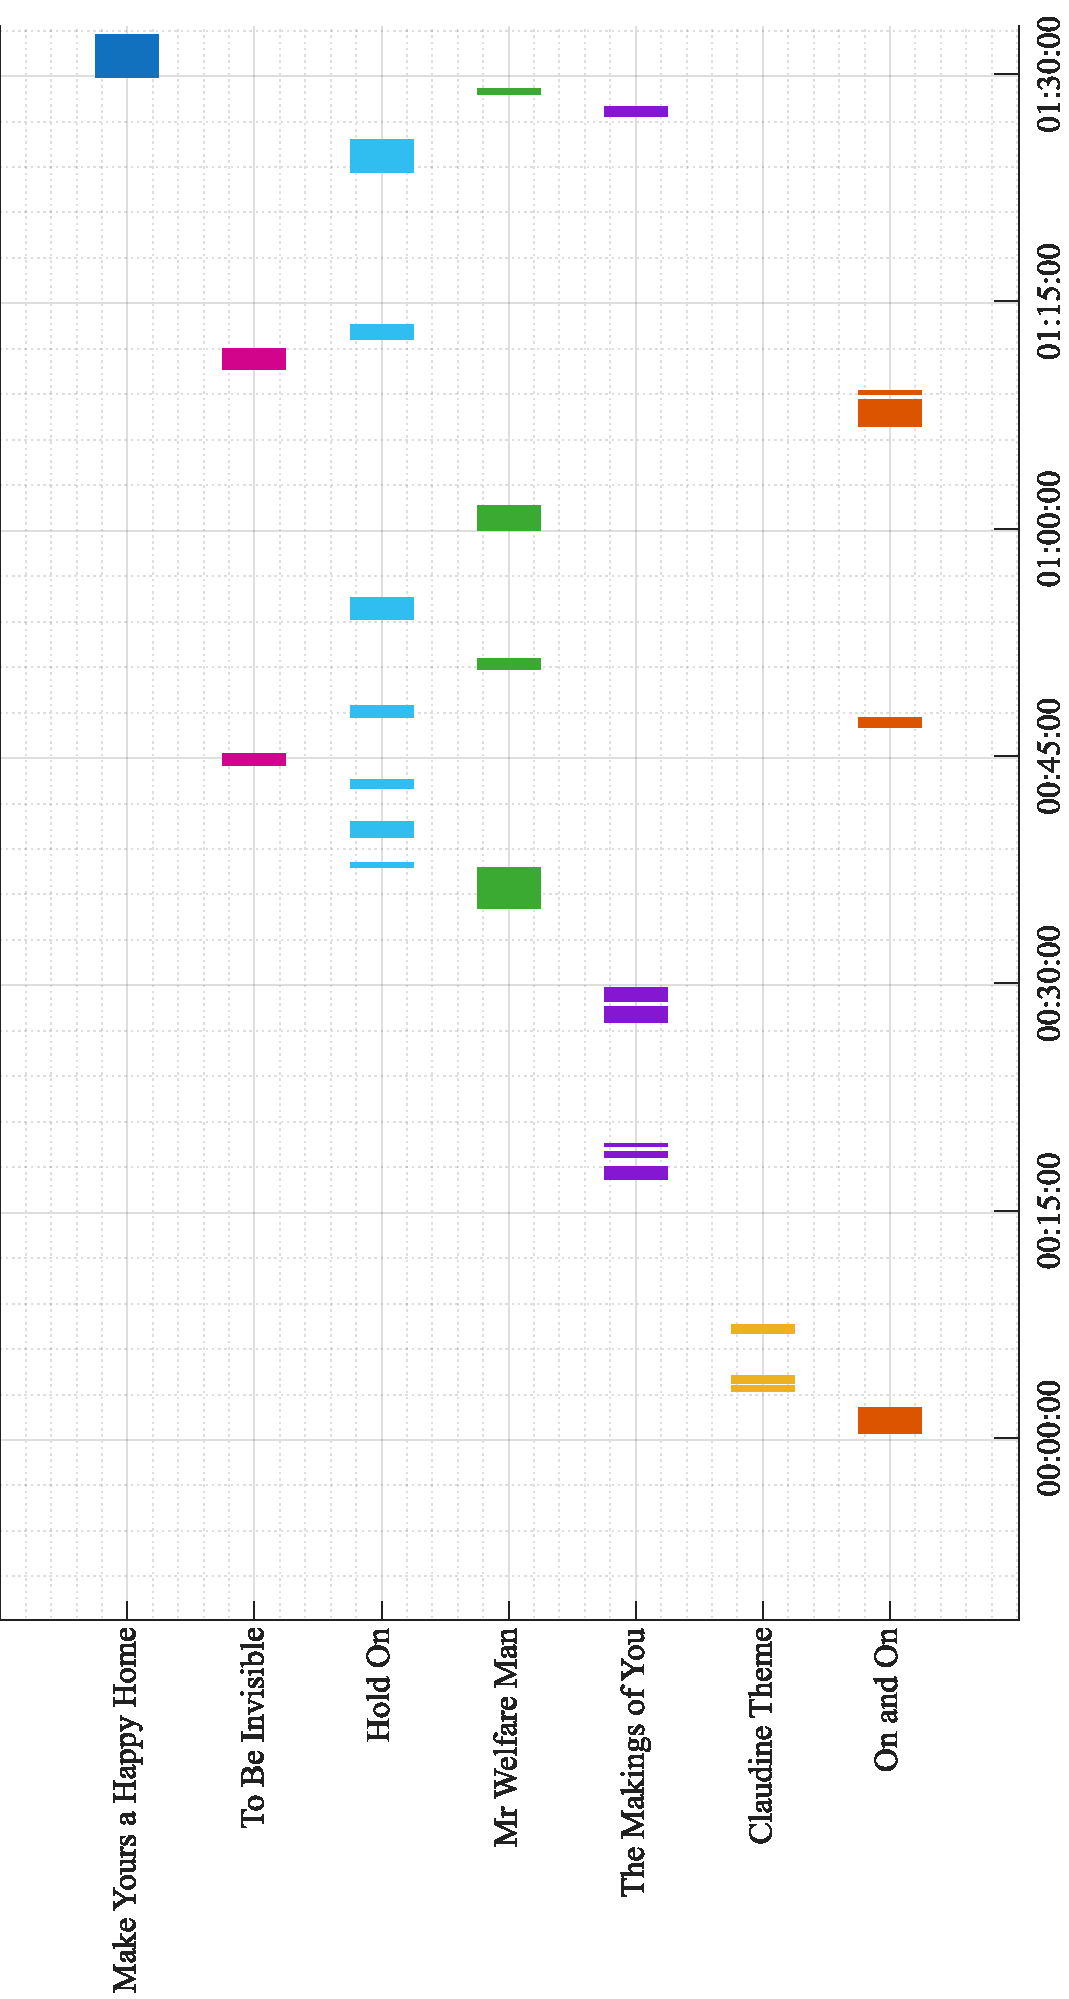
\includegraphics[width=0.75\linewidth]{img/claudine-timeline-songs.pdf}
    \caption{Timeline depicting the placement and duration of the seven songs heard throughout \textit{Claudine}}
    \label{fig:claudine-timeline-songs}
\end{figure}


\textit{Claudine}'s soundtrack follows the trend of many blaxploitation films through the use of soul, funk, and R\&B songs performed by an ensemble typical of these styles with heavy percussion, electric guitars, keyboards, pianos, and brass all featured prominently.
The majority of the songs heard, however, are more sentimental than usually heard on many blaxploitation soundtracks, with the lyrical content typically addressing romantic themes.
These songs therefore provide a deeper emotional resonance in contrast to the more stoic masculinity heard in other films.
This is aided by Knight's voice which imbues the songs with a strong emotionality.

A further similarity is in the songwriting of Curtis Mayfield, who by the early 1970s had become a highly prolific and celebrated composer for films. 
Mayfield himself commented upon the seeming ubiquity of his film scores during this period:
\begin{quote}
I was standing in Chicago right on State Street, the main street in the Chicago theater district, right there in the Loop. And I looked out, and right there I could see the marquee for three of my movies at the same time, Super Fly, Let’s Do It Again, and I think it was Claudine. Right there in my hometown.\autocite[][216]{werner_higher_2004}
\end{quote}
I have discussed Mayfield's work on \textit{Super Fly} in the previous chapter, but it is important to note the ubiquity of similar compositional practices for contemporary, urban-set films.
By this time, it had become common to compose films using either pre-existing or specifically composed popular music.
Although this was not novel to the New Hollywood period, it did not become as widespread until the mid-to-late 1960s. 
With the rise of the predominately white New Hollywood, the music heard was typically rock and roll: modern artists to reflect the rebelliousness of contemporary youth; older artists to evoke nostalgia for a by-gone era.
As Mervyn Cooke notes in his \textit{A History of Film Music}, popular music has been used as an ``ethnic marker" in both music and film industries, and the increase in ``black-oriented" films meant an increase in soundtracks written and performed by black artists.\autocite[Cooke writes that, following the threat of legal by the National Association for the Advancement of Colored People unless more people of colour were hired in the film industry, by 1972 roughly 25\% of US-produced films were ``black-oriented."][401]{cooke_history_2008}
This led to the proliferation of soundtracks from black artists such as Isaac Hayes and Marvin Gaye.

Mayfield's lyrics closely mirror the film's narrative and emotional tenor, and are written in the first-person.
The similarities, and the use of ``I" throughout the soundtrack, gives the impression of representing Claudine's subjectivity.
Other times, though, Knight addresses Claudine directly.
In this way, the music is used as a Greek chorus, commenting on the onscreen action with an apparently omniscient understanding of the film's narrative and the characters' subjectivities.
This latter point is heard in ``Hold On," a slow gospel track in which Knight sings the line, ``Claudine's gotta hold on."
This song reflects Claudine's need to withstand the financial and emotional difficulties she faces.
Other songs address the film's narrative on a more thematic level.
``Mr. Welfare Man," for example, deals with the bureaucracy of the welfare system, while ``To Be Invisible" express the desire to run away from the harsh realities of urban life.

While each of the seven songs heard on the soundtrack were performed by Gladys Knight \& the Pips, some had previously been released before the film was produced.
``The Makings of You," for example, was recorded and released on Mayfield' debut solo album, \textit{Curtis} (1970).
An earlier iteration of Knight's ``On and On" was also released on the Impressions' 1972 album \textit{Times have Changed}, under the title ``Our Loves Goes On and On."
Neither of these tracks were released as singles so it is unlikely that there was much awareness of the songs prior to their use in \textit{Claudine}.
However, \textit{Curtis}, the most commercially successful of these two albums, had reached number 19 of the Billboard pop charts in November 1970 and number 1 of the R\&B charts in February 1971, suggesting that ``The Makings of You" may well have been known by both Mayfield's fans and more general fans of popular music.\autocite[][]{noauthor_curtis_nodate} 
Following the release of \textit{Claudine} in April 1974, Mayfield released interpolations of two other songs from the soundtrack, ``To Be Invisible" and ``Mr. Welfare Man," which appeared on his albums \textit{Sweet Exorcist} (1974) and \textit{Give, Get, Take and Have} (1976), respectively.

The significance of audiences' previous awareness of songs in films is hinted at by Jeff Smith, who explores the use of popular music in film.
As Smith writes, the use of a well-known song in a film creates the possibility that audiences will ``create associations different from those intended by the filmmakers."\autocite[][166]{smith_sounds_1998}
The likelihood of this may well depend on the audiences' experience with the songs used, or the song's subtextual meaning contrasting that of the scene it is accompanying.
Smith goes on to claim that when audiences hear songs they are already familiar with, ``the matter of song lyrics becomes more a question of recognition than cognition. Instead of deciphering lyrics, viewers simply apply what they already know–a title or chorus–to the specific dramatic context that is depicted in the film."\autocite[][166]{smith_sounds_1998}
Upon \textit{Claudine}'s release, it is likely that only fans of Curtis Mayfield and the Impressions would have been familiar with the songs in its soundtrack, somewhat negating Smith's concern regarding their previous associations of the songs contrasting with their use in the film.

This point is further negated through Gladys Knight \& the Pips' role as a Greek chorus, and Mayfield's songs having been either written specifically for the film or rewritten to better suit the film's narrative and perspective.
As such, there is little room for misinterpretation or misplaced associations, since the songs generally match their respective scenes' narrative and emotional subject matter.
In his study, Smith dispels the notion that audiences pay much attention to the lyrical content of popular music in films, as their attention generally remains on the narrative content of the scene.
In the case of \textit{Claudine}, however, some of the songs are heard as the primary feature of a scene's soundtrack, with no diegetic sounds competing for prominence.
Smith's claim that audience attention is not on ``the decipherment of often unintelligible rock lyrics" is here mooted as the the songs become the only aspect of the soundtrack and hence their content is uninterrupted by diegetic, narrative sound.\autocite[][166]{smith_sounds_1998}
Furthermore, the nature of the soundtrack's Greek chorus ensures that the lyrical content of the soul and funk music used in \textit{Claudine} is far more audible and decipherable than the rock and roll that Smith focuses his attention on.

Though the soundtrack features popular music with lyrics that are prominently heard in the sound mix, some sequences are scored with instrumental sections of these songs.
For spectators not familiar with the songs on the soundtrack, it can therefore be easy to overlook the repeated use of certain songs.
With the removal of the lyrics, and Mayfield's prominent use of luscious strings and brass instrumentation, the songs in these sequences are more akin to traditional, instrumental soundtracks of classical Hollywood convention.
However, the presence of more electric timbres and syncopated rhythms, typical of 1970s funk and soul, reflect the film's contemporary, urban setting and reinforce the film's modern sensibilities.

This use of songs allowed the filmmakers to place the film firmly within the contemporary film landscape, while also giving the impression of containing a more traditional, instrumental non-diegetic score.
Mervyn Cooke describes this method of composing a film with both pop music and an orchestral score as ``dual tracking," and though this was not precisely the case in \textcite{berry_claudine_1974}, it remains a useful term when considering how the songs are employed.\autocite[][477]{cooke_history_2008}
Kevin Donnelly writes that dual tracking became a common trend in films in the 1990s, with the pop songs and orchestral score providing different functions: ``the non-diegetic underscore would be designed to elicit emotional effects ... while the pop songs would be an attraction, either foregrounded as non-diegetic music, or appearing only momentarily in the film but available fully outside the film as a tied-in product."\autocite[][153-154]{donnelly_pop_2001}
This suggests that the use of pop songs was primarily commercially-motivated.
Though Mayfield's songs are thematically relevant to many of the scenes they accompany, this financial aspect was undoubtedly a factor in scoring the film in this way.

In each of these aspects, Mayfield's soundtrack follows the trend of many blaxploitation soundtracks which similarly used funk and soul songs, and lyrical content that often commented upon their films' narratives.
Such songs were typically performed by male voices to reflect their predominately male protagonists' masculinity, and contained a grittiness in keeping with the films' emphasis on violence and crime.
Gladys Knight provides a more emotional resonance through her vocal performance and the songs' lyrical content.
This added sentimentality suitably matches \textit{Claudine}'s more grounded narrative and its focus on romantic and family drama.

Despite foregrounding Knight's voice and the more relatable concerns of contemporary life, the perspective that this supposedly brings is slightly undone by the songs' composition by a male songwriter.
As I will discuss below, this problematises the songs' narratives as their perspectives are filtered through a male lens.
For Mark Anthony Neal, this was a common facet of many black popular music:
``unfortunately, many of the musical narratives of the era, given the tremendous commodification of black popular music during the 1970s, were constrained by market limitations that often betrayed black women's agency in their own work."\autocite[][76-77]{neal_what_1999}
Neal's focus here is on the marketing of black female artists, with often included an overt sexualisation at the expense of artistic or political credibility.
While this may not strictly be the case with \textit{Claudine}, Neal's concern remains as the experience and agency of the film's female protagonist is presented on the terms of the film's male composer.



\section{Romantic Comedy Overview}

As we have seen in earlier chapters, narratives around 1960s and 1970s film cites a large shift in the types of films that attracted audiences.
The relaxation of the Hay’s Code, younger audiences, and a rise of audience cynicism regarding the societal and political climate, along with the economic pressures of the major Hollywood studios led to a greater dependency on smaller, cheaper, and more personal films.
The numbers, however, offer a different history.

Between 1967 and 1975–the apparent high point of the “New Hollywood” era–the top grossing films of each year largely speak to audiences’ continued appreciation for “traditional” genres with a generally conservative perspective.
The top grossing film of 1967 and 1968 were \textcite{nichols_graduate_1967} and \textcite{kubrick_2001_1968}, two films that captured contemporary society’s apathy and desire for radical appropriations of conventional genre film.
Following these years, however, the top grossing films domestically were generally less challenging and more standard genre fare:
\textcite{hill_butch_1969}, \textcite{hiller_love_1970}, \textcite{jewison_fiddler_1971}, \textcite{coppola_godfather_1972}, \textcite{hill_sting_1973}, \textcite{brooks_blazing_1974}, and \textcite{spielberg_jaws_1975}.\autocite[][]{noauthor_all-time_nodate}
With the exception of perhaps \textit{The Godfather}, this tells us that, even at the height of the New Hollywood movement, there remained a large audience for crowd-pleasing films that adhered to traditional genres such as musicals, Westerns, crime capers and, most pertinently for my purposes, romantic narratives.

As Leger Grindon notes in \textit{New Approaches to Film Genre the Hollywood Romantic Comedy}, romantic comedies have been one of the most celebrated genres of film since the arrival of synchronised sound.\autocite[][25]{grindon_hollywood_2011}
He notes that while the generic conventions are consistently adapted “to keep the movie fresh,” the fundamental elements remain the same.\autocite[][2]{grindon_hollywood_2011}
These narratives follow the blossoming relationship of the two lead characters, ultimately culminating in their union after overcoming numerous trials and tribulations, thereby providing an equal dose of melodrama and feel-good romance.
In their very nature, romcoms are typically apolitical, and do not tend to overtly address socio-political anxieties.
Rather, as Grindon suggests, they often reflect contemporary societal landscapes and conflicts that supposedly exist between the genders, often with regards to characters’ opposing careers, social status, and regional and religious cultures.\autocite[][4-5]{grindon_hollywood_2011}

Grindon identifies and surveys several cycles that the romcom underwent from advent of sound cinema to the “grotesque and ambivalent cycle” of 1997 to 2011, the year of his study’s release.\autocite[][26-66]{grindon_hollywood_2011}
While some of these cycles are identified purely by era-defining cultural and geo-political events–such as 1930–1933 and the rise of sound cinema, and 1942-1946 and World War II–each cycle represented and responded to contemporary societal desires and attitudes.
Perhaps the most obvious example of this is seen in the “screwball” cycle of the late 1930s and 40s.
During this period the United States was recovering from a severe economic depression, and yet, as Grindon argues, “hope became widespread” due to President Franklin Roosevelt’s economic programmes.\autocite[][32]{grindon_hollywood_2011}
This optimism was reflected in this series of light-hearted, feel-good romantic comedies.

Following the Second World War, however, such optimism evaporated as the nation attempted to adjust to the trauma of post-war reality.
Those who were able to return from the war struggled to acclimate to civilian life, while women were no longer required in the factory jobs they had held in the absence of an all-male workforce, and were instead shepherded back to traditionally gendered roles.
Henry Jenkins discusses the gendered conflicts that subsequently arose: “men felt a perpetual threat to the stability of their masculine authority; while women were beginning to question the normality of traditional feminine roles."\autocite[][253]{jenkins_laughingstock_1995}
In keeping with the national trauma, Grindon notes that the romantic comedies of this period “were haunted by separation, loss, and death.”\autocite[][43]{grindon_hollywood_2011}
Despite the varying tonalities and subtexts, inherent to most romcoms throughout multiple eras is a conservative attitude to heteronormative relations. 
This is also reflected in \textit{Claudine}.


\section{Claudine}


\textit{Claudine} was directed by John Berry, who, after spending much of his early career contracted to Paramount Studios, developed a ``loyal following within the American Black community of the time" due to his work directing stage productions of \textit{Native Son} (Richard Wright) and \textit{Deep are the Root}s (Arnaud d'Usseau and James Gow).\autocite[][210]{hayward_french_2010}
As Susan Hayward writes, these plays both depict ``racial issues and inter-racial relationships."\autocite[][210]{hayward_french_2010}

Berry was blacklisted in 1951 after being named as a communist sympathiser by Edward Dmytryk, a member of the Hollywood Ten.
He was forced into exile in France where he continued to make films, most prominently \textcite{berry_tamango_1958}, which depicts a revolt aboard a slave ship transporting slaves from Africa to Cuba.
He returned to the United States in 1964, directing more stage productions, and remained ``associated with black themes over the next few decades."\autocite[][]{bergan_obituary_1999}
\textit{Claudine} marked his return to Hollywood.
As I hinted above, \textit{Claudine} shows a radically different depiction of life in contemporary New York to \textit{Super Fly}, and highlights the socio-political constraints that many faced within this environment.
It may therefore be best defined as a social problem film within a romantic comedy. 


\subsection{Narrative Overview}

\textit{Claudine} depicts the struggles of Claudine Price, a single mother in Harlem, as she attempts to raise her children while negotiating the strict parameters of the welfare system.
As a welfare recipient, Claudine is unable to hold a job without risking her benefits, and yet is unable to sufficiently care for her children with the money provided to her.

The film opens by literally centring Claudine as she walks down the street in a long shot, flanked by her six children.
The children each kiss Claudine goodbye, as she rushes for the bus to her secret job as a housekeeper for a suburban upper class family.
While at work, she meets binman, Rupert ``Roop" Marshall, and they agree to a date.

That evening, Roop arrives to take Claudine out, but she is home late and suggests postponing the date.
Roop comes into her home and we get an insight into her chaotic family life as her children scream at each other, fight over the use of their single bathroom, and clearly struggle to make do with their small apartment.
Two of the older children angrily express concern that Roop will get Claudine pregnant and leave, as they have seen happen before.
Nevertheless, Claudine and Roop go out for their date at Roop's apartment.
Roop's home seems more comfortable and far less claustrophobic than Claudine's, though he still has to deal with a mice infestation and lives below a brothel, hinting at his own socio-economic situation.
There is some friction when Roop questions why Claudine has so many children, but the date ultimately goes well and the two agree to meet again. 

Throughout the film, Claudine is visited by the social worker Mrs Kabak.
Mrs Kabak makes clear that any supplementary income or gifts that Claudine receives must be declared and deducted from her welfare allowance.
In each of these sequences, the family scramble to hide gifts and new appliances that Roop has given them.
During the first of these visits, Mrs Kabak asks Claudine if she has been dating a man and if he has given her any gifts that should be declared.
Claudine expresses her outrage at what she perceives as unjust regulations that monitor her personal life.

In a later scene, Claudine discusses the inequality of her welfare allowance, likening the ``welfare man" to an abusive husband (00:42:13):
\begin{quote}
I'm married to the welfare man. That's my husband. Makes me beg for them pennies. That starvation money. And if I can't feed my kids, it's child neglect. Go out and get myself a little job on the side and don't tell him, then I'm cheating. If I stay at home then I'm lazy. You can't win. Mr Welfare, that is the nosiest husband in the world.
\end{quote}

In addition to her financial difficulties, Claudine struggles to ensure her children do not fall into the same cycle that she did by avoiding teenage pregnancies and focusing at school.
These concerns are focused on her two eldest children, daughter Charlene who keeps going out with her boyfriend Teddy, and son Charles who joins a black revolutionary gang and risks run-ins with the police.\footnote{In another apparent reference to black revolutionary groups, Teddy changes his name to Abdullah, though he his never shown on screen and his political ideologies are never explicitly expressed.}
Her youngest son, Francis, responds to their difficult family dynamic by telling Roop his wish to turn invisible to escape from reality.
The following scene then sees Roop finding middle child Paul gambling in an alley, having decided to leave school after the teacher told him he had no potential.
Roop uses this game as an opportunity to instil the importance of school to improve Paul's prospects.

The issues facing Claudine and Roop's relationship come to a head when child services track him down and charge him with with backpay for missed child support payments.
He disappears from Claudine's life and plans to move out of the city so that child services cannot find him.
After Charles finds him drunk in a bar and fights him, he changes his mind and reunites with Claudine.
The film ends with their wedding in the Price family's apartment.
The police interrupt the wedding though, looking for Charles who had been at a protest that had turned violent.
Charles is arrested but the Price family refuse to let him go, and they are all put into a police van.
They remain content, finally united as a traditional, nuclear family unit.
The film ends with a mirror shot of the opening sequence where we saw the family walking down the street.
This time, however, they are joined by Roop, symbolising the union of the traditional family unit.



\subsection{Claudine's Themes}

\textit{Claudine} addresses many socio-political issues, most prominently the cruelty of the welfare system.
This is explicitly depicted throughout the film with Claudine's attempts to provide for her children while ensuring she follows the convoluted rules enforced by Mrs Kabak.
Claudine knowingly violates these rules and spends much of the film hiding this from Mrs Kabak.
The film makes clear that she does not break the rule to cynically exploit the system, but because the system is not designed to sufficiently care for the most vulnerable and those in similar positions to her. 
Claudine does not attempt to hide her wrongdoing from her community, suggesting the widespread understanding that in order to survive and care for their families, people are often forced into making these decisions.
The film does not judge Claudine for her indiscretions, but encourages the spectator to sympathise with her situation.

Claudine voices the film's critique of the welfare system in her speech quoted above wherein she concisely surmises its unfairness and contradictory nature (00:42:13):
\begin{quote}
If I can’t feed my kids, it’s child neglect. If I go out and get myself a little job on the side, and don't tell him, then I’m cheating. If I stay at home, then I’m lazy.
\end{quote}

Another key scene sees Claudine and Roop visit the welfare offices to discuss their getting married.
The social workers lay out bureaucratic financial requirements related to marriage, including what they need to declare and the stakes of failing to adhere to welfare regulations.
The scene presents as darkly comedic, with the social workers outlining a series of scenarios that invariably constitute welfare fraud.
\textit{Claudine}'s representation of this theme is both liberally sympathetic to the struggles of the likes of Claudine and Roop, while also conservatively disapproving of governmental overreach.
This curtails Claudine's ability to assert her individual autonomy, and actually punishes her for demonstrating any sense of entrepreneurialism.


In addressing issues surrounding the welfare system, the film deals with the contemporary denigration of those suspected of exploiting the benefits system and, in particular, the image of ``welfare queens."
As Julilly Kohler-Hausmann writes in an historical overview of the demonisation of welfare recipients, the 1970s saw an intense rise in the criminalisation of those deemed to be cheating the welfare system.\autocite[][756-756]{kohler-hausmann_welfare_2015}
Kenneth J. Neubeck and Noel A. Cazenave likewise explore this issue, writing that the number of claimants of Aid to Families with Dependent Children–the benefit that Claudine receives–rose from 3.3 million to 7 million between 1965 and 1970.\autocite[][121]{neubeck_welfare_2001}
This issue is intrinsically tied up with racism, and racist employment and housing practices meant that a disproportionate number of welfare claimants were people of colour.
This contributed to the stereotyping of African Americans, and tensions were exacerbated by prominent politicians.
Ronald Reagan is the most infamous of such figures, and made combatting this perceived threat a key point of many of his addresses.

Although Reagan did not begin to make the figure of the the welfare queen a key issue until early 1976, the spectre of ``welfare cheats" had by then become a commonly denigrated stereotype.\autocite[][]{noauthor_welfare_1976}
\textit{Claudine} was thus released in an environment where the titular character's infractions had become a hot-button issue for many, something that Claudine herself sarcastically references during her first date with Roop (00:20:25):
\begin{quote}
Roop: How'd you wind up with six kids?

Claudine: Well haven't you heard about us ignorant black bitches, always got to be laying up with some dude just grinding out having babies for the taxpayer to take care of? I get 30 bucks apiece for them kids. Oh, I'm living like a queen on welfare!
\end{quote}
By addressing issues surrounding the welfare system, \textit{Claudine} also directly deals with the racial stereotypes that this system forces Claudine and Roop to embody.
Claudine, for example, is dependent on her welfare allowance but can only earn it if she avoids work and does not seek romantic partners.
She is thus in a situation where she \textit{must} remain an unemployed, single mother, exactly of the sort that was demonised by the threat of ``welfare queens."
Roop himself feels forced into the position of absentee father by what he deems exorbitant child support.

Masculinity and patriarchal dominance is also a recurring theme.
This theme surrounds Roop's character arc, and greatly affects Claudine’s relationship with her children and the romantic relationship that drives the film’s plot.
While the masculinity of \textit{Super Fly} was demonstrated in Youngblood's physical aggression, sexual prowess, and calculated stoicism, Roop is a far more affable and sentimental representation of male identity.
He demonstrates patriarchal affection to Claudine's children, offering to buy them treats, empathising with Francis's wish to turn invisible due to feeling like a burden, and attempts to instil the importance of schooling in Paul.

He further distances himself from Turneresque ideals of American ideals by mocking the understanding of financial success.
On his and Claudine's first date, he jokingly uses corporate terminology to discuss their romantic future by likening himself to a business venture before explaining his view on material wealth (00:13:26):
\begin{quote}
Roop: You're wondering, what are the possibilities of continued growth.

Claudine: Roop, how come you settle for being a garbageman? I know you're smarter than that.

Roop: Shoot, I been smarter than any job I ever had. No, you see, I actually avoided success. You know why? Because when you are successful and rich, people envy you and hate you. I want people to love me.    
\end{quote}
In this, he rejects the importance of entrepreneurial acumen.

When Roop displays what could be understood as more Turneresque facets of masculinity, the kind embodied by Youngblood and other blaxploitation heroes, he is ridiculed by Claudine.
In one instance, Claudine suggests they get married but Roop responds negatively as he would need to declare himself to the welfare office, albeit as a ``non-recipient" (00:56:46).
Roop resents the notion that he would have to declare his financial income and assets, and the damage that would have on his pride.
Claudine responds by attacking Roop's stubborn hubris:
\begin{quote}
You men got some crazy ideas about being a man. Fighting, beating up on somebody. That makes you a man, right? Screwing all the broads and making babies. That makes you a man. Big man! Nobody ain't gonna tell Rupert B. Marshall how to spend his couple of little, shitty dollars.
\end{quote}
When Roop drunkenly claims he will leave New York and ``get me a hustle, get some broads," Claudine sarcastically replies, ``your kids are going to love that. `Kids, have you heard? Daddy's gonna be a pimp" (01:05:10).

\textit{Claudine}, does, however, align with \textit{Super Fly}'s apparent attitude toward black revolutionaries.
In \textit{Super Fly}, Youngblood is visited by black revolutionaries who try to get him to contribute to ``building a new nation for black people" (01:02:06).
Youngblood rebukes them and chastises their form of peaceful protests:
\begin{quote}
I'll tell you what you do, you go get you a gun, and all those black folks you keep doing so much talking about get guns, and come back ready to go down, then I'll be right down front killing whitey. But until you can do that, you go sing your marching songs some place else.
\end{quote}
This attitude is reflected in \textit{Claudine} when her oldest son Charles joins a group that protest against the lack of employment opportunities that systematically forces black people to remain on welfare and therefore denies them financial independence, security or social mobility.
Though the group's demands seem to reflect the film's ideology, their more radical means are portrayed as ineffectual.
Claudine mocks Charles for sharing this ideology, hinting at his naivety: ``my son the black revolutionary. You ain't nothing but a snot-nosed coward" (01:13:53).

While Youngblood rejected the black revolutionaries' ideology on account of their being too peaceful, \textit{Claudine} rejects it as being too radical.
This reinforces Michael Ryan and Douglas Kellner’s claim that the mid-1970s saw ``a turn away from the rhetoric of black power and toward a rhetoric of moderation.”\autocite[][121]{ryan_camera_1988}
In direct contrast to the militant, countercultural ideology of \textit{Super Fly}, \textit{Claudine} reflects what Ryan and Kellner describe as an argument ``against radicalism and for an acceptance of the logic of capitalism."\autocite[][121]{ryan_camera_1988}

This can also be seen in the film's production.
\textit{Claudine} was produced by short-lived production company Third World Cinema Corporation, which was established in 1971 to provide opportunities for actors and filmmakers of colour in an industry that they had often been denied access to.\autocite[][]{weiler_third_1971}
The company therefore came at a time when blaxploitation cinema was beginning to amass a large following and cultural footprint.
As Monica Castillo wrote in a 2019 essay in \textit{Film Comment}, ``movies from Third World Cinema (TWC) were to serve as antidotes to those narratives. And Claudine was its success story."\autocite[][]{castillo_divided_2019}
The company therefore represented a countercultural response to the major film companies, while still ``accept[ing] the logic" of the capitalist system that had often refused TWC members entry.\autocite[][121]{ryan_camera_1988}
In this, the film's ideology regarding the callousness of government welfare is somewhat subverted, as much of the TWC's funding came from federal grants.\autocite[][136-137]{lev_american_2010}



\section{Soundtrack Analysis}

The seven tracks on \textit{Claudine}'s soundtrack follow funk, soul and R\&B generic tropes.
These genres share a similar ancestry, and are amalgamations of African-derived techniques and contemporary instrumentation and ideologies.
This provides a contrast to musics coded as ``American," such as that associated with the Western genre, that was derived from European traditions.
I detailed in my study of \textcite{sherman_big_1971} how Western composers sought to define the American identity with a new language of composition.
This involved implicitly drawing upon Turner's notion that the American identity necessitated a rejection of European cultures; to be American meant denying one's more diverse cultural and national background.
Yet, while the likes of Copland and Bernstein took such traditions and attempted to codify an American style of music and national identity, funk music was often more critical of American identity, its ideology, and the notion of ontological essentialism that it celebrated.

An understanding of the ideology of funk and its potential to represent national identities requires questioning Turner's notion that the United States is predicated upon a cultural homogeneity.
Drawing upon African diasporic music traditions, for example, challenges the notion that ``American” should be defined in contrast to ``European.”
By focusing on rejecting European cultural identity, Turner downplayed–or outright ignored–the significance of the presence of non-European identities.
Funk music, on the other hand, represents the diversity of the United States in a way that Western Art Music, by its very nature, cannot.

Furthermore, John H. McClendon III, a philosopher of African-American studies, challenged the Turneresque idea of American homogeneity in an article exploring jazz as a uniquely ``American" practice:
``such judgments are predicated on a cultural philosophy that presumes the United States to be a singular national entity with a corresponding state apparatus, i.e., a nation-state."\autocite[][22]{mcclendon_iii_jazz_2004}
For McClendon, jazz–and by extension its various subgenres and affiliated genres–derived from the African American experience of slavery and inequality.
These musics responded to their practitioners' contemporary environment, drawing upon both North American contexts and African cultural heritage.
This draws implicitly upon Paul Gilroy's prioritisation of ``routes" over ``roots," the suggestion that black identity cannot be defined by its ontological ``root" but by understanding the ``traffic between African cultural forms and the political cultures of diaspora blacks over a long period." REFERENCE.
Matthew P. Brown, drawing upon Amiri Baraka, also discusses this, writing that ``African-American artists call on a tradition rooted in African religious worship; these practices are revised ... in the Christianized world of America."\autocite[][489]{brown_funk_1994}

These genres therefore represented a more complicated and critical understanding of the American national identity, as we can see in Claudine's introduction compared to John Wayne's Jake McCandles.
While Jake was clearly coded as an all-American frontier hero when he was introduced with the Coplandesque fanfare, Claudine's introduction does not feature any such heroic music asserting her essentialist cultural identity.

This reveals a fundamental contrast between the two films' political ideology: \textcite{sherman_big_1971}, and Westerns more broadly, embrace and celebrate the American character codified by Turner, specifically heard through its music; \textit{Claudine} employs musical genres that defy such simplistic national identifiers and categorisations.
For many Westerns, challenging the American character's dominance was perceived as intolerable, with villains often acting as stand-ins for the threats facing American civilisation.
\textit{Claudine}, however, uses its soundtrack in a similar way to many contemporary blaxploitation films which often interrogate ideas of national identity and cultural belonging.
This resulted in the rejection of the apparently intrinsic dominance of (white) American hegemony that Westerns–as well as Turner's thesis–championed.



% Gilroy -  “The specificity of the modern political and cultural formation that I want to call the black Atlantic can be defined, on one level, through this desire to transcend both the structures of the nation state and the constraints of ethnicity and national particularity.”




As detailed above, \textit{Claudine} focuses on several interconnected subtextual themes: governmental overreach with regards to the welfare system; systematic racial inequality; capitalism; patriarchy and heteronormative family dynamics.
Each of these mirror, to some degree, the characteristics celebrated in Turner's thesis, and are referenced either directly or indirectly in the soundtrack songs.
Since the themes outlined above are broad, I will simplify them into the following categories:
capitalism; gender; and community.
This latter theme, while not explicitly addressed, is nevertheless a key subtextual element and provides a contrast with the Turneresque ideal of individualism.
Furthermore, as Angela Davis writes, creating a sense of community has long been an intrinsic goal of black music throughout the 20th century: ``Black people were able to create with their music an aesthetic community of resistance, which in turn encouraged and nurtured a political community of active struggle for freedom."\autocite[][201]{davis_women_1989}
This has also been discussed by musicologist Graham Lock who outlined the desire for an idealised future and communal belonging that is supposedly inherent in many black musics.
Citing a work by Duke Ellington, Lock refers to this future as ``Blutopia":
\begin{quote}
a utopia tinged with the blues, an African American visionary future stained with memories. In this reading of the word, it is the refusal to forget its history that distinguishes Blutopia from other utopian futures. And if that history, largely shaped by the `obscene adventure' of slavery, has made the vision of a better future that much more necessary as an aid to survival, its particular horrors also must have made such a vision harder to sustain, requiring an optimism-against-the-odds (and a means of expressing it) that might be regarded as impossible or even insane.\autocite[][3]{lock_blutopia_2000}
\end{quote}

Table \ref{tab:claudine-songs} provides a overview of the seven songs on the soundtrack, their lyrical content, and musical accompaniment, particularly highlighting the prevalence of community and gender.
The songs are listed in the order that they appear on the official soundtrack release.
I will now discuss the themes of community, gender, and capitalism, with reference to specific songs and scenes as relevant.



\begin{table}[!h]
    \centering
    {\footnotesize
    \renewcommand{\arraystretch}{2.6} % vertical margin
    \begin{tabular}{m{1em}m{0.12\linewidth}m{0.34\linewidth}m{0.34\linewidth}}\toprule
           \multicolumn{2}{c}{Song}& Lyrical Theme& Musical Description\\ \midrule
        1
& Mr Welfare Man
& A critique on the welfare state and the stereotypes that it reinforces among black mothers. Uses the metaphor of being married to the “welfare man” and needing to divorce him to assert independence and stability self-respect.
& A mid-tempo, upbeat funk style. Led by a string melody. Syncopation emphasises the lyrical motif of divorce and the lack of stability ``Mr Welfare" provides.\\ 
        
2
& To Be \newline Invisible  
& Outlines the narrator's desire to be invisible to escape the harshness of contemporary life which is ``so mean" that an individual's humanity is not recognised. Questions the notion that freedom is extended to all while those in positions of wealth and power are granted more respect and dignity.   
& In 3/4 time signature, unlike all others in the soundtrack. Prominent strings add an emotional tenor. An electric guitar adds additional textures through harmonics and volume swells.\\ 
    
        3
& On and On
& Addresses the narrator’s difficult situations but states the importance of love in persevering through such difficulties. 
& Upbeat funk track with organ, electric guitar, bass guitar, drums. Electric guitar is played through a wah-pedal which adds additional percussive quality to the song. \\ 
        
        4
& The Makings of You
& Narrator details their feelings for their partner. Along with “Make Yours a Happy Home,” this is one of the only songs that does not gender the narrator or their partner, allowing it to represent both Claudine’s and Roop’s feelings for each other.
& Slow tempo with a lead string arrangement, organ accompaniment and rhythmic electric guitar. The guitar often responds to vocal lines with a brief lick.\\ 
      
        5
& Claudine Theme
& N/A – instrumental.
& An instrumental funk piece led by string melody. Percussion and an electric guitar played with a wah-pedal add extra rhythmic textures. A bass motif is repeated throughout. \\ 

        6
& Hold On
& Narrator details her male romantic partner’s indiscretions, but chastises herself for not being more forgiving. Encourages herself to “hold on” through the difficult times in their relationship.
& Opens with an extended church organ section before it fades out and is replaced with an ensemble of organ, electric guitar, bass guitar, and drums. Performed in a traditional gospel style but with secular lyrical content. \\ 

7
& Make Yours a Happy Home
& Reiterates the need for a loving home and family life. Acknowledges that, though the narrator’s partner is not perfect, they can overcome any issues. The narrator outlines that making their partner happy is all that matters to them. As referenced above, the narrator and their partner are not gendered, implying that this sentiment could be shared by Claudine and Roop. 
& A sentimental soul piece. Brass instrumentation provides the melodic accompaniment with a string ensemble adding additional melodic flourishes. \\
    \end{tabular}
    }
    \caption{Overview of the seven songs featured on \textit{Claudine}'s soundtrack.}
    \label{tab:claudine-songs}
\end{table}


% \paragraph{Mr Welfare Man:}

% A mid-tempo funk song led by an orchestral string melody.
% The song remains upbeat despite its lyrical content which provides an explicit critique on the welfare state and the stereotypes that it reinforces among black mothers.
% The lyrics reflect Claudine's speech about being married to the ``welfare man” and needing to divorce him to assert independence and stability self-respect.
% Heavy syncopation in the chorus emphasises the lyrical motif of divorce and the lack of stability that the welfare system provides.

% \paragraph{To Be Invisible:}

% A more tender and emotional track, ``To Be Invisible" uses its prominent string melody to add a strong emotional tenor.
% The song also differs in being in 3/4, while all others on the soundtrack remain in 4/4.
% An electric guitar adds additional texture through harmonics and volume swells.
% The lyrics outline the narrator's desire to be invisible to escape from the inhumanity of contemporary life which is ``so mean” that an individual’s humanity is not even recognised.
% Although it is Claudine’s son Francis who wishes to be invisible in the film's narrative, the narrator reverses the gender by referring to ``a girl with no name.”
% This makes the desire to be invisible more universal and less specific to Francis.
% It further questions the notion that freedom is extended to all, while those in positions of wealth and power are granted more respect and dignity.	


% \paragraph{On and On:}

% An upbeat funk track with organ, electric guitar, bass guitar, drums.
% Electric guitar is played through a wah-pedal which adds a percussive quality to the song, typical of the funk genre.
% The narrator details their difficult situation but states the importance of love in persevering through such circumstances.
% Despite the pessimistic tone set by the lyrics and emotionality of Knight's delivery, the music is not melancholic or downbeat.
% The chorus vamps over a static E minor chord, representing the cyclical nature of generational inequality that the film address while a propulsive drumbeat reflects the need for continued perseverance.


% \paragraph{The Makings of You:}

% A love song with the narrator detailing their feelings for her partner.
% It maintains a slow tempo with a lead string arrangement, organ accompaniment and rhythmic electric guitar.
% The guitar often responds to vocal lines with a brief lick.
% Along with ``Make Yours a Happy Home,” this is one of the only songs that does not gender the narrator or their partner, allowing it to represent both Claudine’s and Roop’s feelings for each other.	


% \paragraph{Claudine Theme:}

% This is the only instrumental piece on the soundtrack, though it maintains stylistic similarities with the rest of the songs by remaining with the funk tradition and featuring a prominent string melody.
% Additional percussion and an electric guitar played with a wah-pedal provide extra rhythmic textures.
% A prominent bass motif is repeated throughout, and seems to reference Claudine’s seemingly impossible financial situation.

% \paragraph{Hold On:}

% Perhaps the biggest outlier of the seven tracks, this is performed within the gospel tradition and opens with a church organ, establishing religious overtones.
% The organ fades but is replaced by an ensemble of keyboard, electric guitar, bass guitar, and drums.
% Though the song is performed in a traditional gospel style, particuarly in Knight's vocal delivery and the Pips' accompaniment, its lyrics do not address religion or spirituality.
% The narrator details her male romantic partner’s indiscretions, but chastises herself for not being more forgiving. 
% She encourages herself to ``hold on” through the difficult times in their relationship, implicitly forgiving him for any wrongdoings.
% She also addresses Claudine directly by instructing to also hold on through her own personal struggles.


% \paragraph{Make Yours a Happy Home:}

% A sentimental soul piece, this final song features lead brass instrumentation, while a string ensemble adds additional melodic flourishes.
% The lyrics reiterate the need for a loving home and family life, and acknowledge that, though the narrator’s partner is not perfect, they can overcome any issues.
% The narrator outlines that making their partner happy is all that matters to them.
% As referenced above, the narrator and their partner are not gendered, implying that this sentiment could be shared by Claudine and Roop. 	



\newpage
\subsection{Community}


\subsubsection{On and On}

The sense of community is represented by the Price family, the union between Claudine and Roop, and the musical and lyrical contents of the soundtrack.
It is outlined from the film's opening.

Following the 20th Century Fox logo, the image dissolves to a black screen.
This is held for roughly eight seconds before a cut to an image of New York bridges.
While this black image is on screen, Knight's provides the first sound of the film, singing the third verse of ``On and On." 
She is accompanied by a very quiet electric guitar, making it sound almost a cappella.
The cut to the New York landscape is synchronised with the introduction of Knight's backing group, the Pips, who join in harmony with Knight.
Table \ref{tab:claudine-on-opening} provides a summary of this opening sequence.


\begin{table}[h]
    \centering
    \begin{tabular}{p{50mm} >{\raggedright\arraybackslash}p{50mm}p{50mm} }\toprule
         Lyric&   Visual Action&Soundtrack Description\\\midrule
         How can I work out this sweet relation?&   Black screen&Faint electric guitar\\
         Let us deal with love&   Cut to image of New York bridges&Pips enter, harmonising\\
         Keeping our hearts together&   ``Twentieth Century-Fox Presents"&\\
         With no temptation&   &\\
         Keeping us loving&   ``A Third World Cinema Production"&\\
 Hugging and loving (hugging and loving)&  &Call and response with Pips performing lead vocal and Knight performing response\\
 Getting with the kissing (getting with the kissing)&  &Drums enter playing four-on-the-floor beat\\ \bottomrule
    \end{tabular}
\caption{The lyrics and musical and visual accompaniment from \textit{Claudine}'s opening title sequence. Brackets denote lyrics sung by the Pips.}
\label{tab:claudine-on-opening}
    
    
\end{table}


Knight's vocals are made even more prominent by the lack of visuals, and for the six seconds before cutting to the image of New York, the spectator is left alone with the vocalist.
The opening, questioning line is foregrounded, and the spectator is forced to face the singer's existential dilemma and her confusion.
% We soon come to understand that this sentiment reflects Claudine's emotional state, and the lyric's appeal for love to help overcome adversity foreshadows her relationship with Roop.
% These characters have not been introduced at this point, and yet these themes are established from before the title sequence has even begun.
As we will see in the following chapter, \textcite{pakula_all_1976} starts in a similar way and opens with the abrasive punching of typewriter keys.
The urgency in Knight's vocal delivery introduces the sense of desperation that remains throughout the film.
This is reflected in the call and response vocal exchanges, which begin with her repeating the Pips' lines before descending into non-lexical yells.
These interjections and their emotional tenor contribute to the track's rising tension.
\textit{Claudine}–and, as I will argue, \textit{President's Men}–open by using the soundtrack to layout thematic subtexts before the narratives get underway.

Noted above, ``On and On" is not introduced from its beginning–as it appears on the accompanying soundtrack album–but from the third verse.
The official version is not performed in this near-a cappella style, however; it is here edited to heighten the power and significance of Knight's vocals and the lyrical content.
These combine to present a strong sense of defiance, most overtly heard in the chorus's repetition of the title line, ``on and on."

The drums are added to the mix and the song moves into the pre-chorus with a call and response section.
The Pips repeat the lines ``hugging and love" and ``getting with the kissing" while Knight replies with either a repetition or non-lexical vocals.
The drums perform a steady four-on-the-floor beat while a staccato organ vamps in time with the snare drum.
This leads to a drum fill synchronised with a camera cut to a long shot of a Harlem street as the Price family turn the corner.
Claudine is in the middle of her six children, and the family walk toward the camera as the film's title card appears.
The drum fill introduces the chorus and the full band of electric bass, guitars, and organ.
During this chorus, the Pips repeat the title line on the first beat of every fifth bar while Knight fills the intervening bars with expressive, ad-lib style vocals, reiterating the song's theme of defiance with lines such as ``we gotta move," and ``keep on moving."
As the apparent narrator, Knight's use of the collective ``we" aligns her with the spectator, drawing them closer, and indicating the universal need to persevere through trying times.

The ensemble vamps over the tonic key of E minor, building a sense of tension as the listener awaits a climax that seems to never arrive.
This is exacerbated by the minor tonality
However, although repetition is commonly understood in film music as means to heighten tension and unease–as a I will discuss in my following analysis of \textit{All the President's Men}–as Matthew P. Brown notes, this is a primarily Western tradition.
For Brown, ``the Western tradition concentrates on harmonic, tonal or melodic development," and the lack of this development is often perceived as inherently displeasing.\autocite[][497]{brown_funk_1994}
Funk music, on the other hand, ``looks for no such resolution."\autocite[][498]{brown_funk_1994}
As such, ``On and On's" repeated E minor instead reflects tradition funk aesthetics and, by adhering to these traits, reiterates the genre's theme of personal and political perseverance.

One by one, Claudine's children go in their separate directions, kissing her goodbye who then rushes to catch her bus.
As she boards the bus, one of her sons runs to the doors to give her her bag which she had left with him.
This opening establishes Claudine as clearly overextended, ensuring her children get to school with their correct bags and signed permission slips, while running late herself.
It simultaneously foregrounds the Price family as a close-knit community, each member contributing to taking care of each other, seen in how Claudine's son rushes to give her her bag and how her elder daughters help the youngest daughter to cross the street.
The camera cuts to an interior shot of the bus where Claudine joins her friends, and the song abruptly fades out, replaced with the diegetic sounds of the bus and her friends' voices.

Sung in the first-person, the lyrics seem to detail Claudine's perspective and reflects her own subjective need to ``keep on moving."
This latter point seems explicit as the Pips' first phrase of ``on and on" is heard as the title card fades onto the screen.
While the card is still onscreen, Knight sings her response ``keep on moving, on and on," drawing a direct link with Claudine and the need to persevere.
Though this makes the song specific to Claudine, ``On and On" simultaneously reflects the same need for the wider community.

With its use of call and response, devotion to ``keep on moving" to a better place, and musical repetition, the chorus of ``On and On" exhibits recurring tropes of the funk genre, the former two highlighting the need for community.
Inspection of these traits, and the invocation of community, reveal prominent implications towards questions of national identity.
Call and response is perhaps the most noticeable of these traits.
Knight and the Pips' shared vocals is emblematic of the sense of unity that funk music sought to inspire, outlined by William C. Banfield in his discussion of 1970s funk:
\begin{quote}
driven by an even harder beat, with a bigger dominance of the rhythm section, featuring electric bass, punctuating guitar, drum, synthesizer, and a funky horn section. The music with strong vocal leads revolved around a repetitive drive, syncopated feel, which was created largely to be a social party dance music ... The music was intended to bring people together to have fun.\autocite[][159]{banfield_cultural_2010}
\end{quote}
With the exception of the synthesiser, Banfield's description closely mirrors the aesthetics of ``On and On." 
Following this, the song can be better understood as an attempt to highlight the importance of togetherness, albeit on a more spiritual level than the social level that he cites.
Claudine's position within this community is therefore emphasised.

Within the funk genre, this community was typically black and Afro-diasporic communities. 
This offers a contrast to the music heard within \textcite{sherman_big_1971} and \textcite{parks_super_1972} wherein the music seemed to celebrate and idealise the individualist hero.
The use of call and response and funk music, an inherently communal music, instead prioritises the wider community of which Claudine is a single member. 
Though the song positions Claudine as a microcosm of her community, and thus downplays the fundamental importance of individualism, this is subverted at later points in the film when the music addresses her directly.
I will discuss such instances at a later point.

The combination of musical repetition and defiant perseverance in lyrics, meanwhile, represents what Brown calls the ``paradox of funk poetics."\autocite[][491]{brown_funk_1994}
Brown's assertion is predicated on funk music's ``teleological orientation," which, he claims, consists of a ``will to imagine a future end ... situated within a repetitive, circular, montage-based structure that resists progress and closure."\autocite[][491]{brown_funk_1994}
In this, Brown refers to funk music's lyrical content which typically aspires to a communal transcendence, with regards to both a literal socio-political environment and a more metaphysical spirituality.
This is contrasted with the repetitive, circular nature of the music which seems to never progress or transcend to a triumphant climax.
The chorus in ``On and On" presents this in its vamping over a sustained E minor chord.

Using funk, soul, and R\&B to introduce urban, inner-city environments is a common filmic trope and are standard genres for prototypical blaxploitation films.
This has been explored by Richard Dyer, who discusses the thematic significance of using contemporary funk and soul soundtracks to accompany the opening title sequences of blaxploitation films. 
I have discussed \textit{Super Fly's} opening in the previous chapter, and it is important here to note \textit{Claudine}'s similarities to the opening sequence of not just \textit{Super Fly} but other blaxploitation films such as \textcite{parks_shaft_1971} and \textcite{cohen_black_1973}.

Dyer writes that introducing blaxploitation characters in urban spaces establishes their ``connectedness to this world," and, by extension, their community.\autocite[][156]{dyer_space_2012}
This assertion is also true of Claudine and her family.
The similarity between these films' opening sequences is further highlighted by the use of title cards superimposed over images of the streets and often, although not exclusively, over the first sighting of the films' protagonists.
Figure \ref{fig:claudine-titlecard-comp} compares \textit{Claudine}'s title card with \textit{Super Fly}'s and \textit{Shaft}'s, two quintessential blaxploitation films.
These title sequences are all accompanied by funk music, revealing another similarity between \textit{Claudine} and its blaxploitation predecessors.
As I outlined above, \textit{Claudine} was in essence a response to the aggressive, hyper-masculine crime narratives told in blaxploitation cinema.
Its opening sequence, however, reveals that it adhered to the same stylistic conventions to introduced this urban setting and to portray its protagonist as a member of this community, despite attempting to represent a different, more authentic image of contemporary black life.


\begin{figure}
    \centering
    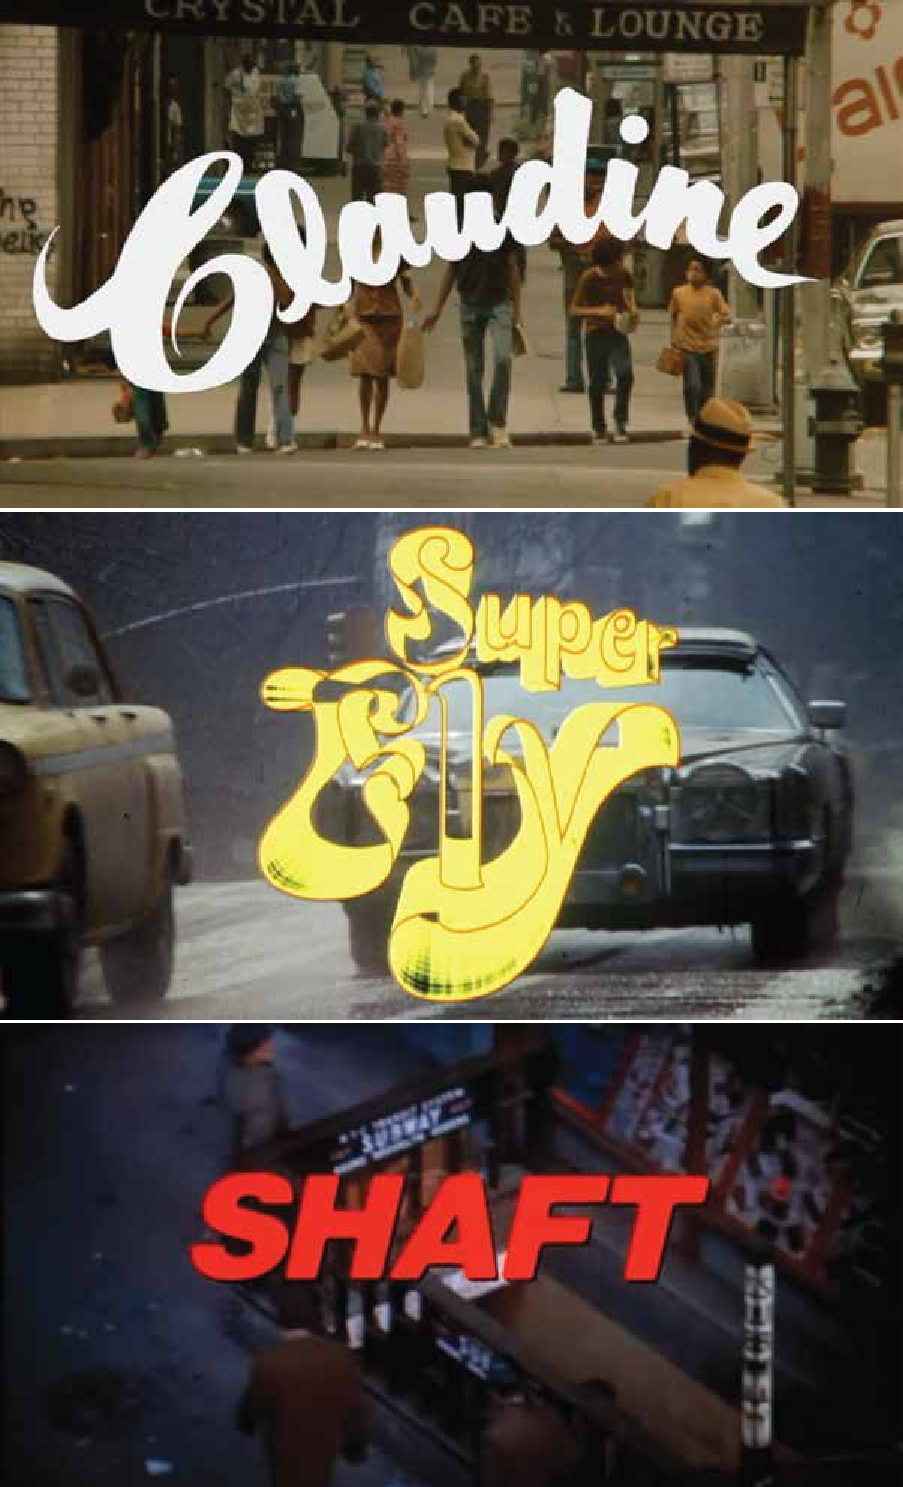
\includegraphics[width=0.5\linewidth]{img/claudine-titlecard-comp.pdf}
    \caption{Title cards from \textit{Claudine}, \textit{Super Fly}, and \textit{Shaft}, accompany images of their protagonists' urban environment, tying them to this space and highlighting their connectedness. Claudine is introduced walking with her children. \textit{Super Fly}'s Youngblood Priest is seen driving his car. And the titular Shaft is seen exiting a subway station.}
    \label{fig:claudine-titlecard-comp}
\end{figure}


Justifying this typical opening sequence seen in many blaxploitation films, Dyer claims that this can be understood a reference to racist perceptions of US inner-cities:
\begin{quote}
proudly affirm[ing] what had long been fixed in the geographical imagination, that the city had already become an African-American space. The perception of `white flight' from the cities to the suburbs and the centrality of the notion of the–now overwhelmingly black–ghetto in imagining cities were now entrenched.\autocite[][158]{dyer_space_2012}
\end{quote}
In much the same way that blaxploitation cinema played with racist ideas surrounding black crime, these opening sequences ``do not seek to counteract such perceptions so much as to own, embrace, celebrate and sometimes interrogate them."\autocite[][158]{dyer_space_2012}
As we see later in the film, this interrogation of stereotypes is fundamental to \textit{Claudine}.

Claudine's connectedness to her urban space is paramount when considering questions surrounding American identity.
By linking her with this urban setting through music and \textit{mise-en-scène}, the film's opening sequence functions in the same way as that of earlier blaxploitation cinema, what Dyer describes as ``musical affirmation and interrogation of black men's belonging in the spaces of America."\autocite[][173]{dyer_space_2012}
With the necessary gender reversal, Dyer's assertion is apt for \textit{Claudine}, and we can understand this opening sequence as associating Claudine with New York, the urban environment and quintessential American city.
Despite connecting Claudine with this environment through music, the sounds of her environment are almost entirely removed from this sequence.

\textit{Claudine}'s opening is played with almost no diegetic sound despite the camera's proximity to passing cars and other people on the street.
The near total removal of diegetic sound seems to remove Claudine from this environment, downplaying her connectedness to this space and community.
It also subverts the film's attempts at creating a ``realist" social drama.
By removing nearly all diegetic sound from the scene, though, the song's theme of perseverance is foregrounded as there are no competing sound effects that might distract the spectator's attention from the song's message.
% It remains the only audible accompaniment, and thus the sequence's signal sound. 

The only break from the song's total dominance of the soundtrack is in a roughly two second interjection where the sound of car horns are clearly heard (00:01:21).
This diegetic interjection is synchronised with the music's return to the verse that opened the film.
The drums return to the four-on-the-floor beat and the vocalists perform the same lyrical arrangement heard before.
The rest of the ensemble repeats a four-bar diatonic chord sequence: \(i\Rightarrow\ III \Rightarrow\ VI\Rightarrow\ iv.\)
% Though this is a somewhat subtle shift, its coinciding with the diegetic sound of passing cars is significant.
As I have suggested above, the music here represents Claudine's subjectivity.
The brief diegetic soundtrack therefore represents an encroachment of the ``real world" into Claudine's interior state and challenges the defiance of the chorus.
Whereas she had previously focused on the need to persevere and ``keeping on moving," the harsh realities of her life are briefly foregrounded and she is forced to face the same existential question that opened the film:
``how can I work out this sweet relation?"

Through all of this, Claudine is presented as defiant in the face of socio-economic hardships.
And though she is coded as deeply connected with her environment, and with a more contemporary image of American identity, the existential dilemmas she faces are foregrounded through the lyrics' opening question.
In response, as the chorus repeats, she persists ``on and on."

Returning to McClendon's and Gilroy's respective arguments cited above, the funk soundtrack highlights the falsity inherent in Turner's thesis: while he may have identified several traits that make one ``American," this thesis requires a very narrow perspective on cultural identity.
Claudine's American identity is established from her first introduction, indicated through her connectedness to her environment and the use of a musical genre that draws upon the diverse historical routes that have shaped the nation's socio-political evolution.
This is achieved in a manner in sharp contrast to the Coplandesque introduction of Jake McCandles, thus challenging the implication that a quintessential ``American" form of music should be derived from a predominately white, Western European cultural practice.


\subsubsection{To Be Invisible}

% people like Gilroy etc. must have written about something like that: not feeling like you fit in so attempting to be invisible.

Another song in which the theme of community is heard is ``To Be Invisible," which is first heard around midway through the film in a sequence where Roop speaks with Francis.
Claudine scolds Francis for slapping his younger sister, and he tries to leave the apartment.
Roop calls to him, though, and tells him to come to him.
Francis moves to the table to draw, but Roop keeps trying to talk with him:

\begin{quote}
    Roop: What you gonna be when you grow up?
    
    Francis: Nothing!
    
    Roop: You gotta do something to make a living.
    
    Francis: I don't know. I want to be invisible.
\end{quote}
As Francis says this final line, he crawls under the table.
Roop gets up to walk over to him and ``To Be Invisible" begins.
A guitar swell synchronises with him rising from his chair as the song fades ins.
Roop sits at the table and continues to speak to Francis while he draws under the table.
An instrumental passage from the song is used here, with  string arrangements and guitar harmonics and swells adding a sweet sentimentality to this sequence wherein we see Roop bonding with Claudine's young son.

Francis tells Roop he is drawing ``a house in the country, a mom and a daddy," but when he shows his drawing it is a blank page as they are invisible.
His ``drawing" of this traditional family unit, Roop's attempts to bond with him, and the song's sentimentality combine to point to a desire for a more stable sense of community than the one the Price family are faced with.

The lack of lyrics do not make the connection explicit, though the theme of escape becomes more obvious in the second use of the song, when Paul and Francis search the city for Roop after he fails to attend the father's day party.
This sequence shows a montage of the boys cycling through the streets, accompanied by the song, this time featuring Knight's lyrics (01:10:34).
While the song literally reflected Francis's desire to be invisible in the earlier scene, it becomes more metaphorical in this sequence with Roop having run away from his responsibilities, disappeared from the Price family's life.
The song dominates the sound mix in this sequence.
Unlike the opening sequence, while the boys cycle through the streets, dodging traffic, the sounds of passing cars are clearly heard in the sound mix.
As I will argue below, the presence of these diegetic sound effects have a thematic significance.
This subtle sonic addition grounds the sequence within the real, lived-in world of the Harlem streets, reinforcing the boys' place and belonging within this community.

Roop's reasons for running away can easily seem selfish, as he becomes overwhelmed with the responsibility of being a father figure to Claudine's children while also providing child support for his own children.
``To Be Invisible," however, does not reflect such selfishness.
Rather, it portrays Roop as a victim of a ``world that's so mean."
% This suggests that the song in this sequence is intended as a reflection of his own subjectivity, representing his own perspective on his situation.
The film's broader theme about the dehumanising effect that the welfare state can have, and the impossibility for one to break out of the cycle of poverty that it keeps people in, mirrors this idea that Roop is a victim of this system that denies him the chance for stability.
Consideration of Knight's vocals further this critique by extending it beyond Roop's personal circumstances.

The lyrics reveal a sense of instability and the perception of the world as a cruel and uncaring place as a key theme.
Knight's vocals detail this explicitly, citing her desire to be invisible to escape this ``mean" world that ``seems not for me."
This reflects Francis's and Roop's own desires.
It is significant, though, that the lyrics specifically cites the narrator as ``a girl with no name."
This gender reversal suggests that the lyrics are not intended as a straight representation of Francis's or Roop's subjectivities, but instead points to a universalisation of the song's themes.
By associating the song within the diegesis with Francis and Roop, but apparently sung from Knight's own perspective, ``To Be Invisible" reflects a desire to retreat from the harshness of contemporary life within this urban environment.


For Francis, the desire to be invisible stems from when he saw ``the invisible man on television," presumably referencing the 1933 film.
Yet, \textit{Claudine}'s socio-political subtext suggests a more pertinent allusion to Ralph Ellison's \textit{The Invisible Man} (1952).
Ellison's novel is told from the perspective of an unnamed black man who settles in Harlem–the same neighbourhood that the Price family live in–and explores themes surrounding black identity in the contemporary USA.
Francis's wish evokes Ellison's prologue, in which he writes ``I am invisible, understand, simply because people refuse to see me ... When they approach me they see only my surroundings, themselves, or figments of their imagination – indeed, everything and anything except me." (PAGE!)
This seems to be internalised by Francis, who perceives himself as unimportant due to the lack of societal care extended to him and his family.
He thus echoes Ellison's narrator's claim that, when invisible, 
\begin{quote}
you often doubt if you really exist. You wonder whether you aren't simply a phantom in other people's minds ... You ache with the need to convince yourself that you do exist in the real world, that you're a part of all the sound and anguish, and you strike outwith your fists, you curse and you swear to make them recognize you. And, alas, it's seldom successful. (PAGE!)
\end{quote}
The narrator of ``To Be Invisible" seems to share this sentiment, lamenting the need to minimise her own autonomy, needs, and wants in order to appease those deemed superior to her: ``I must behave myself / for somebody else / who may have a little fame, fortune and wealth."

Francis, Roop, and Ellison's and Knight's narrators share the same perspective on their undervalued place within society, and express a longing to be a part of a community.
For these figures, individualism is akin to invisibility, and contains an inherent political significance:
whereas the Turneresque ideal celebrates individualism, for a society denied the opportunity to participate in an equal society and ``exist in the real world," this could be perceived as a fundamentally hostile situation.
% Francis, Roop, and Knight \& the Pips–the film's omnipotent Greek chorus–share this desire, making it representative of this section of society more broadly.
By broadening the song's subjectivity, the individual's circumstances are made universal. 
The song is therefore not only about Francis or Roop.
Rather, it is about the victims of structures that deny them social mobility, and, paraphrasing Ellison, refuse to see them.
Crucially, this does not lessen the dramatic impact of the characters' situations.
It instead makes their situations microcosms for a community that the song tells us ``don't mean a thing" to the cruel world.


\subsubsection{Hold On}

Though the majority of \textit{Claudine}'s songs are performed within funk and R\&B traditions, ``Hold On" differs greatly as it is an organ-led gospel song.
Lyrically, ``Hold On" is similar to ``On and On," addressing similar themes, detailing a romantic relationship and its various hardships and difficulties.
% They are both also sung from a first-person perspective.
While ``On and On" makes its theme of perseverance overt through its lyrics, ``Hold On" evokes the same message through its lyrics in addition to this alternate musical style.

Gospel music supposedly originated in Chicago church performances in the early 20th century, and has strong associations with religious sermonising.\autocite[][63]{burnim_gospel_1980}
The gospel of ``Hold On" is stripped of this religiosity, yet retains another key facet of gospel, described by Lawrence Levine as a part of the search of ``the black community for the means of sustenance and identity and survival."\autocite[][189]{levine_black_1977}
The sense of community is heard in the narrator's direct address to Claudine, and also through gospel's associations with cultural and spiritual unity.
The evocation of community in turn evokes what Ron Eyerman and Andrew Jamison call the ``emancipatory potential" of black music.\autocite[][97]{eyerman_music_1998}
Josh Kun similarly discusses this potential, writing that ``everything from field hollers to the beats and breaks of hip-hop has historically functioned as a tool of survival and sustenance and a site of emancipatory hope.”\autocite[][23-24]{kun_audiotopia_2005}
With Knight's motivational lyrics, ``Hold On" fits neatly within this mould and demonstrates her and Claudine's respective aspiration to transcend their current situations to more utopian circumstances.

``Hold On" remains an example of Blutopia through its functioning within the established practice of gospel music, despite not focusing on as severe and existential topics as the artists that Lock analyses in his exploration of the term.\footnote{Lock's focus is on Sun Ra, Duke Ellington, and Anthony Braxton, each of whom championed transcending to a utopian civilisation, based on religious spirituality or inter-planetary travel.}
% While ``Hold On" rhetorically addresses romantic relationships, it remains an example of Blutopia through its functioning within the established practice of gospel music.
By aspiring to this Blutopian ideal, the song echoes the ``memories" of African American culture by drawing upon a musical genre that ``retains the most noticeable African-derived aesthetic features of all" contemporary black musical styles."\autocite[][373]{williams-jones_afro-american_1975}
It further reflects Kun's subsequent description of Blutopia as a means to imagine ``an alternate future without relinquishing the black past."\autocite[][24]{kun_audiotopia_2005}
Claudine is encouraged to ``hold on" through the emotional hardships she is enduring, with the promise of a better future, while simultaneously holding on to what Kun describes as ``the black past."
This is achieved while the song also functions within, and is shaped by, a contemporary American landscape, evidenced through its use in Claudine's specific spatial circumstances and socio-economic situation.

``Hold On" thus reflects the past, present, and idealised future of the individual, her community, and the nation as a whole, foregrounding the black American experience and rejecting the idea that Europe is the sole ``foreign" influence from which the United States evolved from.
The Turneresque historical understanding of the United States is here challenged in what can be described as a post-nationalist perspective, which challenges the assumption of cultural homogeneity and white patriarchal dominance, and the rejection of foreign influence.
Rather, we can hear a \textit{celebration} of this influence, and the situating of a distinctly non-Turneresque characteristic ideal.
This effectively presents an alternative ``American" ideal that acknowledges the routes outlined by Gilroy and foregrounds the experiences of female characters within the contemporary societal landscape.


Though the lyrics explicitly address romantic relationships, it is first heard instrumentally when we see Claudine alone in her apartment late at night (00:37:40).
The sequence opens with a shot of Claudine watching over her children sleeping in bed.
She hears a car parking outside her window, and walks to the window to look outside, accompanied by the song's sustained church organ introduction.
Her daughter Charlene enters the room and the song fades out.

Charlene admits she has been out with a boyfriend and has been drinking.
Mother and daughter have an argument in the hallway before Charlene is sick in the toilet.
The shot cuts to them in Claudine's bed with another of her daughters, Patrice.
With this cut, ``Hold On" is reintroduced and we hear an instrumental verse passage.
Claudine and her daughters discuss her relationship with Roop, and Claudine reveals her uncertainty regarding her future with him:
\begin{quote}
    Patrice: You love Roop, mama?
    
    Claudine: Honey, I stopped using that word a long time ago.
\end{quote}{}

It is heard again in the next scene, when Claudine is with Roop in his bedroom (00:40:43).
The song from the previous sequence fades out with the cut to this scene, which opens with a shot of Claudine deep in thought.
The camera pans to show Roop watching her.
He notices that something is bothering Claudine and attempts to cheer her up, to which she replies by detailing issues with her children.
They discuss the state of their relationship and joke that Claudine is married to ``the welfare man," repeating the lyrical theme of a song heard earlier in the film, ``Mr Welfare Man," which I discuss later.

``Hold On" plays after her speech detailing the injustice of the welfare system cited above.
As the scene comes to an end, we hear Knight's vocals on the song for the first time, stating the song's theme of defiance: ``everyone should know, I wanna hold on / Claudine's gonna hold on."
The Pips' backing vocals repeat the phrase ``hold on," reiterating the importance of this message to both the song and the film.

At this point, Knight alters the subject of the song from the first-person ``I wanna hold on," to the third-person, ``Claudine's gonna hold on."
This is the first time that Claudine's name has been mentioned in the soundtrack, and the first time that Knight \& the Pips seem to take on the role of a Greek chorus, commenting upon the narrative and revealing a seeming omniscience regarding her emotional state and future decisions.
This also problematises previous understandings of the musical accompaniment as essentially acting as Claudine's internal subjectivity.

The three songs with lyrics that have been played to this point–``On and On," ``The Makings of You," and ``Mr Welfare Man"–are each sung from the first person and reflect Claudine's personal situation.
They therefore give the impression that the soundtrack is presenting her interiority.
The mention of Claudine by name, however, makes it necessary to interrogate further whose point of view the songs are depicting, and the issue of ``focalisation."
Coined by Gérard Genette, focalisation determines from whose perspective a story is told.
It can be internal–wherein a story is depicted as from a particular character’s consciousness–or external–when the ``hero performs in front of us without our ever being allowed to know his thoughts or feelings."\autocites[][190]{genette_narrative_1980}

The previous understanding of Knight's voice as representative of Claudine's interior state suggested that we are hearing instances of internal focalisation, providing us a privileged insight into Claudine's emotional perspective.
Addressing Claudine directly, however, draws a firm distinction between the narrator and the protagonist, while Knight's use of the first-person implies that she remains a character within the narrative.
This positions Knight as an ``omniscient narrator," who ``knows more than the character, or more exactly \textit{says} more than any of the characters knows."\autocite[][189]{genette_narrative_1980}
Genette identifies this type of narration as ``nonfocalised," as the narrator–existing within the film's non-diegetic soundtrack–seems to exist within this diegetic world, addressing Claudine, and sharing her own woes.\autocite[][189]{genette_narrative_1980}

Perhaps of greater significance, though, is the diegetic status of Knight's narration.
Genette also discusses this in his chapter exploring uses of ``the voice," wherein he interrogates the distinction between first-person and third-person narrators.
With the exception of the one instrumental track, ``Claudine Theme," each of the songs on the soundtrack are sung from the first-person perspective, which inspires the reading of the songs as representative of Claudine's point of view.
Invoking her name denies the plausibility of this reading.
Genette offers two terms useful for such circumstances: heterodiegetic, where an omniscient narrator tells the story and is not a presence within the narrative; and homodiegetic, where the narrator is also a character within the narrative being depicted.\autocite[][244-245]{genette_narrative_1980}
Knight's first-person lyrics imply her position as a homodiegetic narrator, and though we may initially have understood these lyrics as representations of Claudine's thoughts, the narrator here is placed \textit{within} the narrative.
Knight becomes a character undergoing similar relationship woes as Claudine.
A firm distinction is drawn between Claudine and the narrator as Knight shifts the focus from the first-person ``I" to the third-person ``she."
For Genette, this transition represents a ``glaring violation" of narrative logic and understanding, while ``establish[ing] between the narrator and character(s) a variable or floating relationship."\autocite[][246]{genette_narrative_1980}
This relationship between the narrator and the protagonist–Gladys Knight \& the Pips and Claudine, respectively–highlights the importance of community within this world.
This presents a contradictory attitude to Turneresque individualism that championed in the frontier thesis and was supposedly an inherently American trait.

Rather than prioritising the heroics and experiences of an individual, the individual's connectedness to community is highlighted through the use of both first- and third-person narration which makes Claudine's lived experience appear more universal without downplaying the significance to her personally.
Mark Anthony Neal discusses a similar use of music in Marvin Gaye's compiled soundtrack for \textcite{dixon_trouble_1972}.
In these songs, Neal writes, Gaye sings from a first-person perspective, thereby ``conflat[ing] the personal with the communal."\autocite[][68]{neal_what_1999}
Neal goes on to write that this conflation is a key aspect of many genres of ``black music," and was partly inspired in the late 1960s and early 1970s by the ``erosion of communal discourse within the African-American community."\autocite[][65]{neal_what_1999}
This assertion is appropriate in the case of ``Hold On"; instilling this sense of community is a key aspect of the song and underpins each of the scenes that it accompanies.
For instance, we hear this song again after the gambling sequence described above when Roop and Paul are walking away from the game.
Paul asks what is happening between Roop and his mother (00:47:32).
Roop deflects the question and instead uses the moment as an opportunity to teach Paul about the importance of his education, improving himself and his community.
The sequence therefore sees them bonding and forging a communal, familial connection.

Soon after this scene, the song plays while Claudine and Roop are lying in bed discussing their relationship again (00:54:01).
``Hold On" plays softly in the background but fades when Claudine tells Roop that she thinks they are ``coming to the end of this project."
This synchronisation suggests Claudine has ultimately decided to no longer hold on to their relationship.


The song's final occurrence is towards the end of the film, where Charles finds Roop drunk in a bar (01:22:10).
Charles hits Roop as revenge for leaving Claudine, and the fight concludes with Roop grabbing Charles and hugging him.
``Hold On" begins as the two embrace and continues when the scene cuts to Roop parking his car outside Claudine's apartment.
Claudine and Roop speak in his car and Roop states his plan to leave New York.
The song fades as the children come out and he explains to them that he is leaving for a job in another city.
The children can tell he is lying, though, and he comes to realise that he wants to stay with the family, despite the financial pressure that they are all under.

The idea of community is foregrounded in each of these sequences, represented in the romantic relationship between Claudine and Roop, and in the traditional family unit where the two adults nurture and teach the children important life lessons.
This community is clearly found in the family unit.
The individual ideal is somewhat downplayed here, and yet the traditional values surrounding the nuclear family remains.
These scenes therefore suggest that what Claudine needs to hold on to is this conservative familial ideal, implying that she also must accept her position as secondary to her male partner.
Gender dynamics are a key theme throughout the film, revealing a conservative ideology surrounding the position and autonomy of women.
I now move on to this final theme to explore how this is heard in \textit{Claudine}'s soundtrack.



\subsection{Gender}

\subsubsection{Mr Welfare Man}

Gender is perhaps most overtly discussed in ``Mr Welfare Man."
This is a key song in the film, its title indicating its overt theme of the inhumanity of the welfare system, and this is reflected in the fact that it is second most heard song, occurring four times for roughly 5 minutes and 30 seconds.\footnote{In the fourth of these occurrences, we hear the song's instrumental ending which differs greatly from the verses and chorus sections heard previously. It is therefore difficult to recognise in its final occurrence to those unfamiliar with the song.}
Each of these occurrences are when Claudine is dealing with representatives of the welfare system, usually her social worker Mrs Kabak.

The first time it is heard, Roop is discussing his new relationship with Claudine with his colleague at work.
His colleague warns him to be careful not to get caught or else Claudine could lose her allowance and he would be responsible for her and her children (00:34:55).
A drum fill then introduces the song and four bars of the string motif are played before a cut to the interior of Claudine's home.
She is ironing when one of her sons tells her Mrs Kabak is coming to visit them.
The family jump to action, hiding various items around the house that were gifted to them by Roop, as Mrs Kabak would deduct their value from Claudine's allowance.

The song is placed at the foreground of the sound mix, with diegetic sound effects minimised to emphasise the song's thematic significance.
The lyrics closely mirror Claudine's personal perspective, and detail the situation that she, as a single mother, has been placed in.
Table \ref{tab:claudine-welfare-kabak} details the visual action that accompanies the lyrics in this sequence.
After Mrs Kabak enters and the lyrics in table \ref{tab:claudine-welfare-kabak} are heard, the chorus returns and the vocalists repeat ``keep away from me, Mr Welfare."
Mrs Kabak enters the room and Claudine tells her children to turn down the music.
The song's volume is then reduced, revealing the song as diegetic, and it continues to faintly play throughout the remainder of the scene.
% The song's volume is reduced when Claudine tells the children to turn off the music, suggesting that the song is placed within the film's diegesis.

\begin{table}[h]
    \centering
    \begin{tabular}{>{\raggedright\arraybackslash}p{50mm}>{\raggedright\arraybackslash}p{50mm}>{\raggedright\arraybackslash}p{50mm}}\toprule
 Lyrics& Visual Action&Soundtrack Description\\\midrule
         (Keep away from me, Mr Welfare)&  Claudine and Charlene hide their modern items in the kitchen and replace them with older ones.& \\
         They just keep on saying I'm a lazy women&  & \\
         Don't love my children and I'm mentally unfit&  & \\
         I must divorce him, cut all my ties with him&  & \\
         Cos his ways they make me say&  Claudine moves in to the living room& \\
         It's a hard sacrifice (hard sacrifice)&  Claudine and Charlene roll up a rug placed in the centre of the room.& \\
         Not having me a loving man&  Charles hides the rug behind the curtains.& \\
         Society gave us no choice&  The doorbell rings& \\
         Tried to silence my voice&  & \\
         Pushing me on the welfare (on the welfare)&  Charlene opens the door and tells Claudine Mrs Kabak has arrived.& \\
 I'm so tired, I'm so tired of trying to prove my equal rights& Claudine tells Charlene to let Mrs Kabak in.&Music is lowered in sound mix to allow for Claudine's voice to be heard.\\
 Though I've made some mistakes for goodness sakes& Mrs Kabak enters and greets Charles.&\\
 Why should they help mess up my life?& Charles leaves the apartment, ignoring Mrs Kabak.&\\ \bottomrule 
    \end{tabular}
    \caption{The lyrics and visual accompaniment of the first occurrence of ``Mr Welfare Man." Brackets denote lyrics sung by the Pips.}
    \label{tab:claudine-welfare-kabak}
\end{table}

The song is heard again in an almost identical sequence shortly after this scene, though this time Roop is present and must hide from Mrs Kabak (00:50:34).
At this point, though, it does not feature any lyrics and we only hear an instrumental passage; however, coming so soon after the previous sequence, we are able to recognise the song and its thematic significance.

The song's lyrics foreshadow Claudine's speech, which happens in the following scene, when she complains about being married to the ``welfare man."
It closely resembles Claudine's personal situation, citing her lack of opportunities (``society gave us no choice / tried to silence my voice / pushing me on the welfare"), and the racist stereotypes surrounding ``welfare queens" (``they just keep on saying / I'm a lazy woman / don't love my children / and I'm mentally unfit").
This racism and sexism is directly referenced when Knight sings that she is ``so tried of trying to prove my equal rights," referencing her position as a black woman in contemporary society.
In addition to these issues, Knight details the ``hard sacrifice" of ``not having me a loving man," seemingly equating this lack of romantic partner with the racist structures that deny upward social mobility.

The similarity between the lyrical content and Claudine's situation makes it easy to suggest the song is sung from her perspective; however, the use of ``us" suggests that this is not the case.
Rather, similar to songs discussed above, this positions Knight's narrator, Claudine, and myriad other women in near-identical situations: trapped in a cycle of poverty, in part due to the support systems that are ostensibly intended to help them.
This again marks the importance of community–rather than individualism–and critiques the systemic misogyny that reinforces this subjugation of woman, particularly single mothers.
The music's syncopation likewise reflects the instability that these figures are faced with by denying a steady, rhythmic grounding.

In the second of these sequences, Roop is caught by Mrs Kabak and the scene ends in an argument between the two.
Mrs Kabak explains the regulations surrounding Roop's gifts and support he gives to Claudine.
Claudine scoffs at Mrs Kabak's notion that welfare is ``supporting" her, and states the indignity of needing to ``hide my man in the toilet."
Mrs Kabak's response reveals the societal expectation of heteronormative family dynamics at this time:
``Mrs Price, we want to help, believe me. We know that children need a man in the house, a woman needs a man in the house."
Roop claims the idea that an unmarried man and woman living together is ``immoral," but justifies his current living situation with Claudine by stating that he ``ain't the government."
This reveals Roop's own conservative ideals surrounding family dynamics and the moral righteousness of the government.

Mrs Kabak, as a representative of the government, voices the patriarchal ideology indicative of the Turneresque ideal.
Yet the film's sympathies for Claudine–made evident through ``Mr Welfare Man"–make clear that this is intended as a critique of such regressive and rigid ideals, and of government overreach.
Nevertheless, the sequence and its musical accompaniment outline the contemporary societal expectations of women within the family dynamic, explicitly stating the need for a male figure to provide income and stability.
A similar sense of female subjugation is heard in ``Hold On," the song heard most often on the whole soundtrack.



\subsubsection{Hold On}


As I have detailed above, ``Hold On" focuses on the narrator's relationship troubles, in a gospel-style arrangement.
The narrator complains that her partner is often ``looking out the side of his eye / at every girl who passes him by," and that ``like everyone else, we fuss and fight."
The film's ideology surrounding gender inequality is somewhat subverted here, however, as the narrator appears to subjugate herself to her male partner.
She excuses his transgressions, for example, by claiming that her ``man is the same as every man in the world," and chastises herself by claiming that she's ``asking too much."
Each of the verses end with the proclamation that the narrator wants to ``hold on" to their partner, despite their misdeeds.

This seems inconsistent with the film's ideology regarding the unjust expectations of women when compared to men.
For while ``Mr Welfare Man" seemed to aspire toward empowerment, autonomy, and equality, ``Hold On" appears to instead downplay the female narrator's emotions and expectations in subservience to her male counterpart.
As I argued above, the use of the homodiegetic voice implies community and suggests that this female subjugation is widespread and societal.


The song returns in a sequence shortly after the father's day party that Roop does not attend.
Claudine visits Roop's place of work but cannot find him so returns home and we see her sitting on the steps of her apartment block (01:12:41).
During this sequence, Knight sings adoring lines about how their romantic partner is ``so sweet and he's so kind," implying that despite his behaviour she remains in love with him and is prepared to take him back as soon as he comes back to her.
This ultimately proves to be the case when Roop returns–after being confronted by Charles in a sequence also soundtracked by ``Hold On"–and immediately reconciles with Claudine and her children.



Despite \textit{Claudine}'s textual critique of Turner's patriarchal vision of American identity, ``Hold On" places the narrator and Claudine in a largely deferential role to their respective male partners.
By excusing, justifying, and anticipating her partners' indiscretions, Knight's narrator seems to position herself as subordinate to the man, reinforcing the traditional gender dynamics condoned by Turner.
The song does this by using the individual's relationship as a microcosm for the wider society, thus implying a gender imbalance within domestic relationships.
This can subsequently be seen in Claudine's willingness to forgive Roop of his misbehaviour.

If viewing the song from this perspective, it is important to reiterate that the song was written by the male songwriter Curtis Mayfield.
It is of course impossible to know if the song's narrative would have been similar had it been written by a female songwriter.
Regardless of such hypotheticals, the song's implied gender subjugation contrasts with the depiction of Claudine throughout much the film.
For, while she does ultimately forgive Roop of his wrongdoings, she is never as deferential as the narrator here seems to suggest.
The song's ideal of patriarchal dominance is therefore dissonant with the film's more contemporary depiction of independent female autonomy.



\subsubsection{Happy Home}

%Be more explicit in the film's suggestion that all is well with a complete family unit.

Their reunion is soundtracked by the final song, ``Make Yours a Happy Home."
This plays in the final sequence, Claudine and Roop's wedding in Claudine's apartment
Parallel editing shows that it is placing place while Charles is attending a protest demanding ``jobs not welfare."
Police arrive at the protest after it turns violent and an instrumental version of the bridge of ``Mr Welfare Man" is played.
This funky, trumpet-led passage shares similarities with themes heard in blaxploitation films, echoing Charles's efforts at establishing himself as a revolutionary hero akin to many blaxploitation figures.\footnote{Examples can be found in \textcite{parks_super_1972} (01:21:54) and \textcite{moses_willie_1973} (01:07:35), both of which feature sequences in which their protagonists are chased by police that are similarly accompanied by syncopated funk songs with prominent trumpets, and guitars performed through a wah-pedal.}
Charles is chased by the police, accompanied by this dramatic, action-style section of the song, before the camera cuts to the wedding and the song abruptly stops.

The ceremony continues until Charles enters the apartment, followed by the police.
The police attempt to seize Charles but Roop wrestles them off him and the party descends into a brawl as ``Makes Yours a Happy Home" begins.
Charles and Roop are put in a police van, and Claudine forces her way on board.
The credits begin to roll as a reverse shot shows Paul and Francis running to join the family and getting inside the van as the family are reunited.
The scene cuts to a recreation of the opening sequence where we see the Price family walking down the street.
This time, they are joined by Roop, all smiling, and holding hands.
The image of this happy, heteronormative family is in direct contrast with the first sequence where they were not holding hands or smiling, the colour grading was darker, and one by one they went in separate directions.
During the ending, as the family walk toward the camera, the camera gradually becomes more focused on Claudine's smiling face until showing a close up of her and the film fades to black.
This suggests that, following the union between Claudine and Roop, the family has become a more stable, stronger unit.
Figure \ref{fig:claudine-ending-opening} shows and contrasts the difference between these two sequences.

\begin{figure}
    \centering
    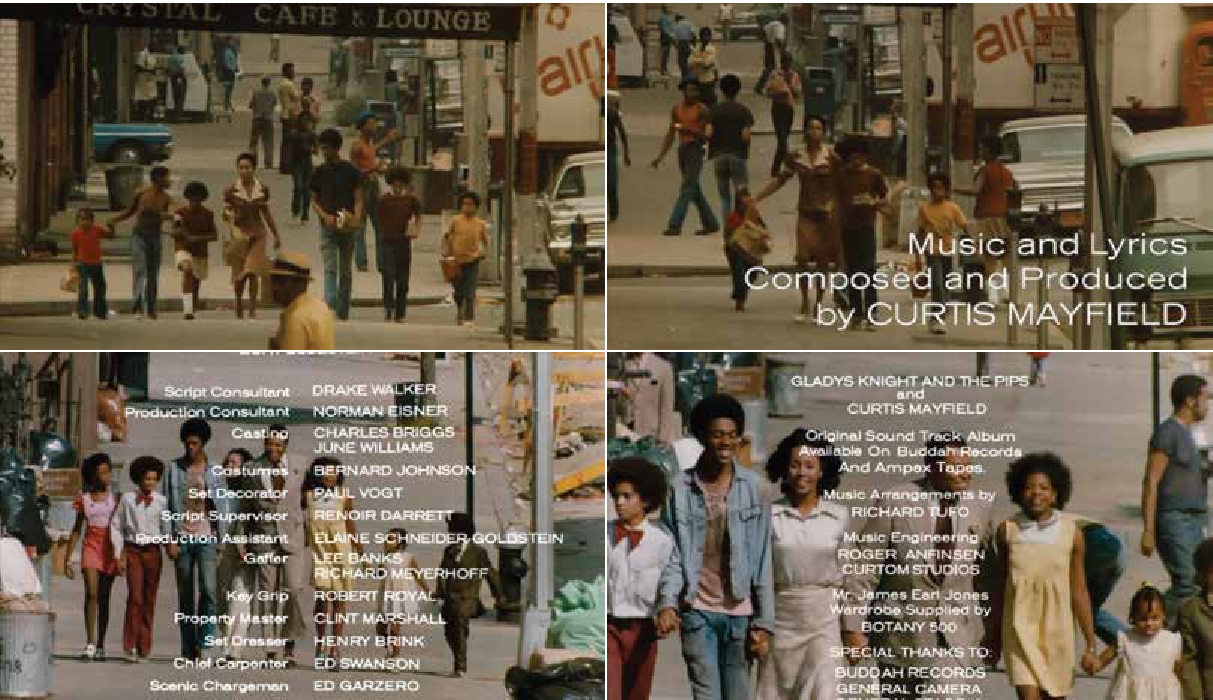
\includegraphics[width=1\linewidth]{img/claudine-ending-opening.pdf}
    \caption{\textit{Claudine}'s opening credits sequence (top right and top left), contrasted with its end credits sequence. The film's conclusion depicts the family as a happier, more stable unit, reflected in their smiles, united line, and the brighter light.}
    \label{fig:claudine-ending-opening}
\end{figure}

The song joins the soundtrack at roughly at its midpoint, with 20 seconds of an instrumental, string-led passage.
Knight's vocals then join with the final line of the fourth verse before moving into the chorus: ``no superstar / I love you just the way you are / so make yours a happy home."
These lyrics crystallise the song's meaning, the narrator expressing her desire to forge a stable and happy family life with her partner.
As the song is only heard during the wedding sequence, the implication seems that marriage is necessary for a happy home.

As was the case with ``Hold On," the narrator makes clear her willingness to subordinate herself in order to please their partner.
This is exemplified as the family are placed in the police van as Knight sings ``I wanna do you right, love me out of sight / I wanna be what pleases you / so long is there is peace with you / that's all I can do."
These lyrics demonstrate the narrator's dedication to her partner, mirroring Claudine's willingness to be arrested along with her new husband.
They also, however, continue the previous theme of female subjugation; the narrator's own emotions and best interests are downplayed in order to prioritise the male partner's.


\subsection{Capitalism}

\subsubsection{Rolling Dice}

\textit{Claudine}'s capitalist themes are alluded to at several points as characters discuss their escape from their socio-economic situations, and the soundtrack regularly reflects this.
It is perhaps most explicit when Roop finds one of Claudine's sons, Paul, gambling when he should instead be in school (00:45:07).
The scene opens with Roop approaching Paul rolling dice under a bridge.
Paul appears to be winning at the game, accruing a large sum of money.
Roop attempts to speak to Paul about him not wanting to go to school, which Paul ignores, focusing instead on his game.
As he rolls the dice, Roop continues to speak about Paul's schooling: 
\begin{quote}
Roop: Teacher embarrassed you in front of the class. Says you didn't have no math potential.

Paul: [Rolls a six and a two] Eight is the point!

Roop: Yeah, I sure hate to see a young fella missing out, not seeing all the good possibilities.

Paul: Possibilities, man? Better myself, make money. Come on, dice! [Rolls dice] The only guys you see with money in their pockets are pimps and the number runners.
\end{quote}
It is unclear whether Paul aspires to be one of the ``pimps and the number runners," but he nevertheless demonstrates admiration for their financial gain.
This scene is used to show the potential pitfalls for those in neglected urban environments, with Paul casually discussing criminal activity that seems to be completely normalised.
He loses on his next roll and Roop outlines the legal and financial risks of such criminal activities, ``after the fines and the payoffs and the time in jail, shoot! They're lucky to have enough money to eat off."
We already understand \textit{Claudine} as a response to the blaxploitation genre, and this exchange is an explicit critique of the genre's apparent celebrating of criminality.
Roop rolls the dice and wins some money while telling Paul about the importance of education, ``not for the money" but for the ``possibilities."
``On and On" is reintroduced in the soundtrack when Roop rolls his first dice.
In this sequence, Roop is trying to instil in Paul the need to improve oneself in order to improve one's personal situation, overcoming the obstacles that prevent his upward socio-economic progression, reflecting the theme of perseverance in ``On and On."

The sound of ``On and On" differs from the title sequence as an instrumental section is used here.
With no lyrics to explicitly state the song's meaning, the song becomes more malleable and its significance reflects Roop's lesson about upward mobility.
While the lyrics in the title sequence implies Claudine's obstacles were related to romantic relationships, Paul's obstacles are his difficult upbringing and lower socio-economic standing.
Roop's belief is clear that with hard work, perseverance, and the drive to push ``on and on," such progress is possible.
In other words, Roop is encouraging Paul to fulfil the entrepreneurial duty of a Turneresque American.

The lack of lyrics might make recognising ``On and On" difficult for those unfamiliar with the soundtrack.
Though it is difficult to measure audiences' prior awareness of music, given the song's relative chart success–peaking at number 5 on the US Pop Charts and number 2 on the US R\&B Charts–it is likely that many viewers would have recognised the music.
As noted above, this attempt at commercial success was likely a factor in using a popular music score, and the song's final occurrence in the film seems an attempt to broaden its appeal, further demonstrating the filmmakers' ideology regarding the purposes of a film's music.



\subsubsection{Party Scene}

The final time that ``On and On" is heard is during a party scene that essentially functions as the beginning of the film's third act (01:06:46).
In this sequence, Claudine and her children are throwing a father's day party for Roop.
After spending much of the film trying to earn the trust of Claudine's children, this party is a significant progression in their relationship.
The scene opens with a shot of Claudine's apartment, full of guests and a large banner reading ``Happy Father's Day."

``On and On" begins with the abrupt edit from the previous scene, opening with the same verse that opened the film.
However, the full ensemble is heard and the scene begins midway through the verse, omitting Knight's question, ``How can I work out this sweet relation?"
The song's existential despair is therefore somewhat diminished.
A more uplifting message of love and hope is presented instead: ``let us deal with love / keeping our hearts together / with no temptation / keeping us loving."

We are therefore hearing the exact same piece of music that was played during the opening sequence, albeit beginning at a slightly later point.
Unlike the opening, however, the diegetic sound of Claudine's guests are clearly heard.
As Claudine walks through the party topping up drinks, her children Charles and Charlene both comment on Roop's absence.
The song fades out as Charlene asks Claudine directly what she's going to do since Roop does not seem likely to arrive.
Claudine snaps back at her and walks to the stereo where she puts on a record.
``On and On" then begins anew, making its placement within the film's diegesis evident.
Her guests begin dancing again while Claudine, standing by the stereo and facing the camera, attempts to join in, her face revealing her disappointment in Roop's absence. 

Though we see Claudine playing the song on her record player, it does not open from the song's actual opening, but from the pre-chorus.
The drums perform the four-on-the-floor beat, the melodic instruments vamp on the E minor chord, and the Pips sing the ``hugging and loving / getting with the kissing" refrain heard in the title sequence.
The paradoxical circularity of funk music is thus reintroduced; the utopian idea of perseverance and overcoming adversity heard in the lyrics is contrasted with the music's repetition.
Claudine becomes inspired by the song's defiant message, joining her guests in dancing to the song, until she is seemingly struck by this circularity and abruptly stops dancing.
She seems to have realised that Roop is not going to come.
After lingering on Claudine's disappointed face, the scene cuts abruptly to her front room, empty except for Claudine and her children.

On a literal level, ``On and On" is presented in this sequence as a fun and upbeat song.
Claudine's guests clearly want to dance to the track so much that she plays the song twice in a row and fills the dance floor.
The song was released as the first single from the soundtrack album, and this sequence can be seen as an effort to establish it as a song well-suited for party and celebrations.
In an essay published in the \textit{Criterion Collection}, cultural theorist Mark Anthony Neal described the song as becoming a ``house-party anthem," and while he does not cite evidence for this claim other than the single's chart success, its use in this sequence is an obvious attempt at instilling this reputation in the audience's imagination.

The soundtrack in this sequence is therefore a clear effort at increasing the film's profits, and an example of filmmakers aspiring to heighten capitalist gains.
Although this does not entirely negate the film's otherwise progressive subtext surrounding race and economic inequality, it does reflect a more conservative and, perhaps somewhat cynical, ideology.
Despite the notion that funk and its adjacent genres represent a more diverse and progressive understanding of American identity, in using it in this way, Turner's vision of American capitalist ingenuity is evident.
% Although being released as the first, and most successful, single from \textit{Claudine}'s soundtrack, ``On and On" is only the third most played song, taking up roughly 4 minutes and 27 seconds of screen time.
% The song featured in most amount of screen time–7 minutes and 21 seconds–was curiously not released as a single at all, ``Hold On."

This is not the only instance where music is suggested at being diegetic, as ``The Makings of You" and ``Mr Welfare Man" are also played on characters' record players.
``The Makings of You" is the most overt example, heard during Claudine and Roop's first date.
While Claudine is in the bathroom, the camera shows Roop take a record from his collection and a cut shows a close up of him putting the record on.
The camera cuts to a medium shot of him and the song begins, making explicit that the song is coming from his stereo.
In keeping with this suggestion, as Roop moves around his apartment–opening the fridge, closing the curtains–the noises he makes are clearly heard alongside the song.

Though showing Roop setting up the vinyl and pressing play can be seen as an effort to create a certain sense of verisimilitude, closer inspection of the shot of the record reveals a clear violation of diegetic boundaries.
Perhaps the most glaring violation is the record that Roop puts on the record player which appears to be a pressing of \textit{Claudine}'s soundtrack.
Figure \ref{fig:claudine-makings-record} shows the close up of Roop's vinyl on the record player beside an image of the original pressing of the soundtrack.
While the exact writing on Roop's vinyl is difficult to read, ``Buddah Records" and the label's logo can clearly be seen. 
Furthermore, he appears to place the stylus toward the end of the record.
This is notable as ``The Makings of You" was the final song on the soundtrack's side A.


\begin{figure}
    \centering
    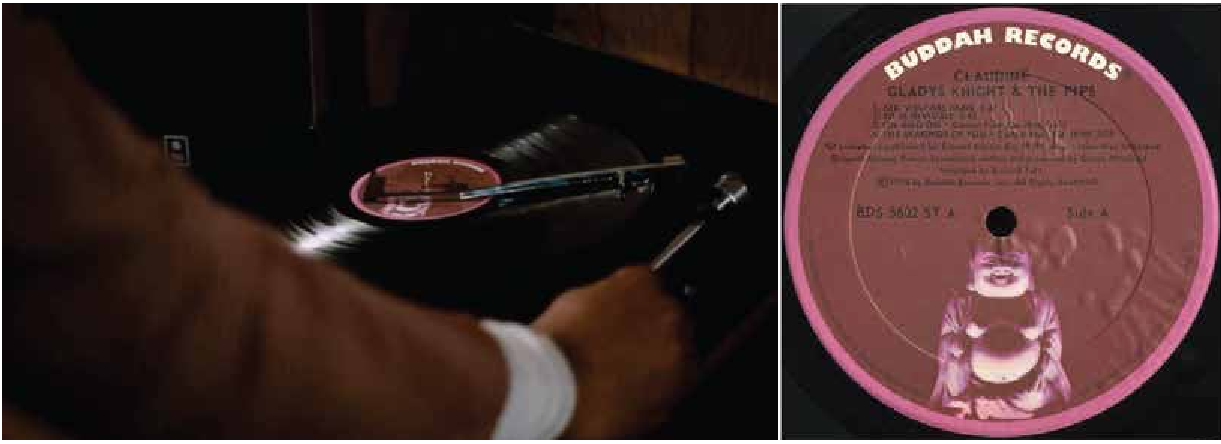
\includegraphics[width=1\linewidth]{img/claudine-makings-record.pdf}
    \caption{Left image depicts Roop setting up his record player. Right image shows the original 1974 pressing of the \textit{Claudine} soundtrack.\autocite[Image of record is taken from a listing available at HHV Records][]{noauthor_ost_nodate}}
    \label{fig:claudine-makings-record}
\end{figure}

This presents a significant, if subtle, reference to the soundtrack as a commercial product, made clear by how Roop places the record with its label clearly facing the camera.
Roop is thus seen handling a key element of the cinematic apparatus, drawing attention to the film's artifice.
The artifice is heightened with Roop's illogical placement of the record player's stylus at the very end of the record's grooves, and how the record does not spin when he switches on the stereo and the song starts.
The song is also not played from its opening as it is heard on the official soundtrack, the opening six bars having been neatly edited out of the film version.

This blurring of diegetic boundaries is a common filmic occurrence, though it most regularly occurs in comedy films.
Marcel Bouvrie, for example, discusses an instance in \textcite{allen_bananas_1971}, when the protagonist opens his wardrobe to find the source of music the spectator had been led to believe was non-diegetic.
Though this is far more overt than Roop's ownership of \textit{Claudine}'s soundtrack, Bouvrie's analysis remains apt in both cases: ``this brief and bizarre moment suddenly pulls the rug out from under the established storyworld and we are suddenly granted a peek behind the curtains of the apparatus of cinema as the film mocks its own conventions and clichés."\autocite[][103]{bouvrie_self-aware_2023}
Bouvrie later discusses comedy films that mock the use of popular music as a cross-promotional tool within the film industry, such as \textcite{jones_monty_1979} which ends with a diegetically performed song before the titular character addresses the camera to remind audiences that the song is available for purchase.
Such cases bring ``the world in which the soundtrack exists as a commodity into the storyworld in order to expose some of the commercial strategies of the film industry."\autocite[][115]{bouvrie_self-aware_2023}
Though not as overtly comedic, \textit{Claudine} stands as another example.
This ``peek behind the curtain" foregrounds the film's artifice and reframes the soundtrack as a commercial commodity, existing outside of the film's internal diegesis.


% The decision to place the record in this way and to not show it spinning suggests a deliberate decision to foreground the film's artificial nature.
Genette calls this exposure of filmic artifice ``metalepsis": an ``intrusion by the extradiegetic narrator or narratee into the diegetic universe."\autocite[Genette adds that this ``intrusion" can also occur in the opposite direction. Although his focus is on literature, his terminology remains useful in this instance, particularly when understanding Knight's voice as akin to a narrator.][234-235]{genette_narrative_1980}
For Genette, this represents a blurring of two worlds: ``the world in which one tells [and] the world of which one tells."\autocite[][236]{genette_narrative_1980}
As I have suggested above, \textit{Claudine}'s soundtrack presents instances of subversion of this dichotomy.
Some of its songs seem unambiguously non-diegetic, some are demonstrably performed within the diegesis, while ``Hold On" exists between these two realms, evident in how Knight addresses Claudine directly.
When understanding Knight and the Pips as essentially the film's narrator and Greek chorus, we can extend Genette's two world binary to include the world \textit{in} which one sings and the world \textit{of} which one sings.
Roop's metaleptical handling of this record thus brings Knight from the former world into the latter.

By highlighting the film's artifice, its ``realist" nature is subverted, if only subtly. 
We are then faced with the notion that, though Roop and his apartment are fictions, the song we hear is real, existing diegetically \textit{and} extradiegetically.
The intrusion of the extradiegesis into the diegesis is seemingly explained by the intention to remind the spectator of the soundtrack as a tangible, authentic commercial product.





% we can see that the record DOES NOT move - artifice of the film as product = artifice of the American identity?
% % Camera lingers on the static shot of the record which is facing the camera, clearly showing the ST on the table.
% Not having the record move was a choice - argue that choice was intended to linger on the record as a product.
% % Breaks the diegetic/4th wall basically.
% % Placement of the stylus is nonsense.
% The song is not at the beginning
% Super-diegetic - when the song exists in both diegetic and non-diegetic spaces. Like in musicals. The character sings within the diegesis but the music exists outside of it. Hogg discusses re. conservative musicals, when characters play a radio and dance along; ``acquires extraordinary abilities, including an omnipresence of consistent volume and quality, regardless of a character’s proximity to the source." 155.

With the understanding that Roop seems to own a copy of \textit{Claudine}'s soundtrack, we can posit that Claudine herself has a copy, based on the party scene described above wherein she plays ``On and On" for her guests.
Her copy seems to be played in an earlier scene as well, during the first of Mrs Kabak's visits.
As I detailed above, the song plays as the family hide the gifts from Roop.
When Mrs Kabak enters, Claudine tells her children to turn their music down and the song's volume is reduced.
It continues to play as Claudine and Mrs Kabak speak for the rest of the scene, and ends roughly two seconds before the cut to the next scene as they both stare at each other.

Since the children turn down their record, and this is synchronised with the lowering of the song's volume in the mix, we are led to believe that the song is coming from within the diegesis.
However, its volume is not consistent with the record player's placement within the diegesis or any of the characters' point of audition.
Again, this acts to remind the audience of the soundtrack as a commodity.

The uses of these three songs arguably counter the film's representation of Claudine's impoverished community by exposing the film's market-driven motivation.
Although the film depicts and empathises with the societal injustice that the Price family are victims of, and critiques the government's fiscal conservatism that holds Claudine in place, it simultaneously demonstrates a desire to exploit this narrative for financial gain.
This is evident in how two of the three songs heard diegetically–``On and On" and ``The Makings of You"–were released as singles in an obvious attempt to increase revenue for the film.
How the songs are heard in the film also acts as an example for audiences on the social and political situations in which these songs are appropriate: ``The Makings of You" is suitable for romantic occasions; ``Mr Welfare Man" can be used to remonstrate against governmental overreach; ``On and On" can be used to fill a dance floor at parties.
As the first, and most successful, single, it seems appropriate that ``On and On" should be heard in this context, as it encourages audiences to perceive the song as a popular, crowd-pleasing song.
% By seeing Claudine seemingly owning a copy of ``On and On," and filling the dance floor when playing it at her party, the spectator is obviously led to perceive this song as a popular, crowd-pleasing song.

To some extent, this is the case for all films that use popular music scores, as commercial potential is a key factor is the decision to score a film in such a way.\autocite[Jeff Smith explores this in depth in this study of popular music in film soundtracks. Discussing compiled soundtracks, he notes that, ``derived from a complex mix of music, marketing, and cinema, the compilation score attained its importance as a commercially self-aware alternative to the neo-Romantic orchestral scores of Hollywood's `Golden Age.'" He later adds that ``the compilation score offered a couple of commercial advantages over its predecessors," primarily ``more potential hits to which the film could hitch its wagon."][155-156]{smith_sounds_1998}
\textit{Claudine} differs from this, however, by blurring the boundaries between the diegetic and extradiegetic worlds when Roop is shown handling the soundtrack.
% That sequence therefore acts as an advertisement for the song and its potential in social gatherings. 
The Turneresque devotion to capitalist progress is thus reflected in a far more obvious manner than contemporary popular music-scored films.
\textit{Claudine}, despite critiquing multiple aspects of this conservative ideal of American identity, therefore demonstrates its obvious financial motivation, not just for its score but for the film more generally.




% NARRATION/PERSPECTIVE

% The narrator's ``presence" is key in correctly identifying homodiegetic narratives.
% As Genette notes, however, ``absence is absolute, but presence has degrees."
% This ambiguity of presence is particularly relevant in film, as the soundtrack narrator seems function within both diegetic and non-diegetic spaces.

% ``absence is absolute, but presence has degrees. ... within the homodiegetic type [there are] at least two varieties: one where the narrator is the hero of his narrative ... and one where he plays only a secondary role, which almost always turns out to be a role as observer and witness." 245 Genette.


% to this point we thought knight was providing internal focalisation. This song seems to involve the ``glaring violation" because we thought Knight's ``I" was essentially Claudine (to this point, we have heard ``on and on", Claudine's theme which is instrumental and ``the makings of you" which is diegetic at first but generally a love song and reflects Claudine's falling for Roop). But in the same verse she sings ``I" \textit{and} ``Claudine" so they are not the same person.
% We are thus presented with Knight as an objectively separate observer, either a secondary witness like Watson, or a representation of heterodiegetic narrator.


% Narrator is placed \textit{within} the story as she here directly addresses Claudine by name, whereas before she was simply singing relevant messages. Knight becomes homodiegetic:
% Makes the subjectivity weird - we have earlier assumed music is her perspective, internal focalisation, essentially. But by mentioning her by name makes clear that it cannot be her internal focalisation; we are hearing someone else's perspective and this person also knows Claudine's interior.


% EUROPEAN CULTURE

% A key point about the rejection of European cultures as American - Turner argues that American identity came after the rejection of Euro culture and the creation of a new one. But alterative lies in how black identity derived from african influence, fused with european. E.g. blues/jazz/etc openly took influence from both to create a new form of identity expression.


% COMMUNITY

% WALD
% "anechoic chamber was an environment that all but banished call and response, rendering listening solipsistic and individualized rather than dynamic and communal." - implication of community in black music communities.





\section{Conclusion}

In \textit{Claudine}, we are presented with an image of American identity in opposition to the figures celebrated in \textit{Big Jake} and \textit{Super Fly}.
A large part of this was intentional on the part of the filmmakers and producers, as the Third World Cinema Corporation sought to present a more positive, realistic, and grounded depiction of life than that shown in blaxploitation cinema.
By shifting the narrative focus away from the traditional, rugged, individualist male hero, \textit{Claudine} argues that the characteristics championed by Turner are not all essential to embody the American identity.
An alternative vision of this identity is presented in the film's narrative and soundtrack.

Mayfield's songs, as sung by Gladys Knight, address this specifically in their lyrics, which focus on Claudine's emotional, financial, and political position within the broader society.
Most obviously, this is heard in the female perspective that Knight's voice offers, despite the songs having been written by a male songwriter.
This presents an alternative perspective and perhaps an inevitable consequence of the prioritisation of patriarchal individuality:
while men are encouraged to embrace their autonomy, and pursue their individualist freedom, in the case of \textit{Claudine}, this leaves the female partners in a far more precarious situation.
The perspective that Knight's vocal provides suggests that Claudine's situation is not unique, as she address herself in the first-person and Claudine directly, making their shared expressions more universal.
The songs therefore seem more motivational and uplifting, despite the seemingly dire circumstances that the lyrics describe, as Claudine is implied as belonging to a supportive and nurturing community.
Knight's group, the Pips, provide an additional sense of community through their backing vocals which further critique the notion that individualism is strictly required and inherently commendable.

Their use of call and response is of course a characteristic of the funk and soul music tradition that the soundtrack functions within.
These genres further critique the Turneresque American ideal in a slightly more abstract way, by opening embracing influence from African and Caribbean diasporas.
Openly drawing upon African and Caribbean cultures reminds listeners of the white supremacist ideology at the heart of Turner's rejection of European cultures.
For while he wishes to surpass these roots, his implication is that the American identity is solely based upon that white, western European diaspora, implicitly rejecting the notion that other continents have contributed to the building of the United States and the shaping of its national identity.

While \textit{Claudine}'s soundtrack displays critiques of Turner's thesis, it still retains some aspects of it.
This is most evident in the subjugation of the female narrator in some songs, wherein Knight's lyrics downplays her own emotional needs to prioritise her male partner's, while also forgiving his indiscretions and chastising herself for expecting better.
Another example is in the commercial aspirations of the popular music soundtrack.
The use of ``On and On" in a party scene, for example, essentially acts as an advert for the song as we see how popular it is among Claudine's friends, as it instantly fills the dance floor.
The literal placement of the soundtrack within the diegesis is a more subtle suggestion of this, but nevertheless acts to remind the spectator that the soundtrack is a commercial product available for purchase and suitable for various social occasions.
Despite the film's textual critique of the callous welfare system and its inherently capitalist ideology, \textit{Claudine}'s soundtrack remains a clear demonstration of capitalist ingenuity, using its socio-political messages to sell a commercial product.




% GENDERING
% the use of the female voice instead of curtis's points to an obvious subjective gendering of the S/T.
% However - Makings and Make Yours DOT NOT include any references to gender so they could represent either C or R. The female vocal does imply it's C, but still an important point.
% The songs that do gender narrator are sometimes written quite deferentially which implies a gender imbalance.







\clearpage
\printbibliography [title=Bibliography,nottype=video]
\printbibliography [title=Filmography,type=video]

\end{document}